%!TEX root = ../my_thesis.tex
\section{Fit validation}
\label{sec:timefitvalidation}

\subsection{Check of nuisance parameters}

The values of the nuisance parameters obtained in the fit (production/detection asymmetries, flavour tagging calibrations) are compared with available
external measurements.

The production asymmetry $A_{\mathrm{P}}$ is compared with the \lhcb~measurement of
Ref.~\cite{LHCb-PAPER-2016-062}. The production asymmetry is computed by weighting
the production asymmetry measured from this paper in bins of $\pt$ and $\eta$,
$A_{\mathrm{P},i}$, with the signal fractions $\varepsilon_i = \frac{s_i}{\sum_j s_j}$
in each bin $i$ of $\Bz\to\Dmp\pipm$ data,
%
\begin{equation}
	A_{\mathrm{P}} = \sum_i \varepsilon_i A_{\mathrm{P},i},
\end{equation}
%
where $s_i$ is the sum of the \emph{sWeights} in bin $i$. This yields
%
\begin{equation}
        \label{eq:prodAsymm}
	%  \begin{split}
	A_{\mathrm{P}} =  -0.0100 \pm 0.0047\,\text{(stat)} \pm 0.0004\, \text{(syst)},
	%  \end{split}
\end{equation}
compatible within 0.65~$\sigma$ with the value obtained from the $\Bz\to\Dmp\pipm$ decay-time fit.

The detection asymmetry $A_{\rm D}$ is also obtained from Ref.~\cite{LHCb-PAPER-2016-062},
and is measured using $\Bz\to J/\psi K^{*0}$ to be $0.0098 \pm 0.0046$ and
$0.0056 \pm 0.0030$ for \num{2011} and \num{2012}, respectively, and using $\Bs\to\Dsm\pip$ to be
$0.0143 \pm 0.0086$ and $0.0103 \pm 0.0058$ for \num{2011} and \num{2012}, respectively.
The central value obtained from the fit to $\Bz\to\Dmp\pipm$ is in agreement with this set of results.

The values of the parameters of the tagging calibrations are compared with those found in the control samples
as described in Secs.~\ref{sec:tagging:OScalib:calibration} and~\ref{sec:tagging:SScalib:combo}. The strategy presented in Sec.~\ref{sec:tagging:strategy} is followed, 
and no perfect portability of the calibrations is assumed a priori, as Sec.~\ref{sec:tagging:OScalib:portability} has shown this not to be the case.
However, the parameter values found in the signal fit are expected to be similar to
those from the control channels given in Tables~\ref{tab:oscalibparams} and~\ref{tab:calibrationSScombination}. 
A full comparison with a $\chi^2$ test that takes into account the correlation between
the parameters is performed. The discrepancy (corresponding to the
$\chi^2$ minimum) is around \SI{0.91}{\sigma} for the OS tagger, and \SI{0.29}{\sigma} for the SS tagger. The parameters which present the largest disagreement are
$\Delta p_{3}^{\rm OS}$ for the OS tagger and the $\Delta p_{0}^{\rm SS}$ for the SS tagger.

\subsection{Fits in data subsamples}
\label{sec:timefitsplits}
A check of the stability of the results against the different data taking conditions is performed by repeating the
fit in four subsamples of the data, namely data taken with magnet ``up'' and ``down'' polarities, and data taken in 2011
and 2012. The \emph{sWeights} for each subsample are obtained via the mass fits described in Sec.~\ref{sec:split}.
The detailed results of these time fits are reported in Appendix~\ref{app:timesplits}. A comparison between the
fitted values for $S_f$ and $S_{\bar f}$ obtained in each subsample is shown in Fig.~\ref{fig:year_pol_splits}.
In all cases, the parameters are in agreement and have good $p$-values, the smallest being the one between the values of
$S_{\bar{f}}$ from the magnet polarity splits (2.7\%). In addition, the average between the fitted
values in each split (black line in Fig.~\ref{fig:year_pol_splits}) is always very close to the central value from
the nominal fit (red hatched band).

\begin{figure}[htpb]
  \begin{center}
    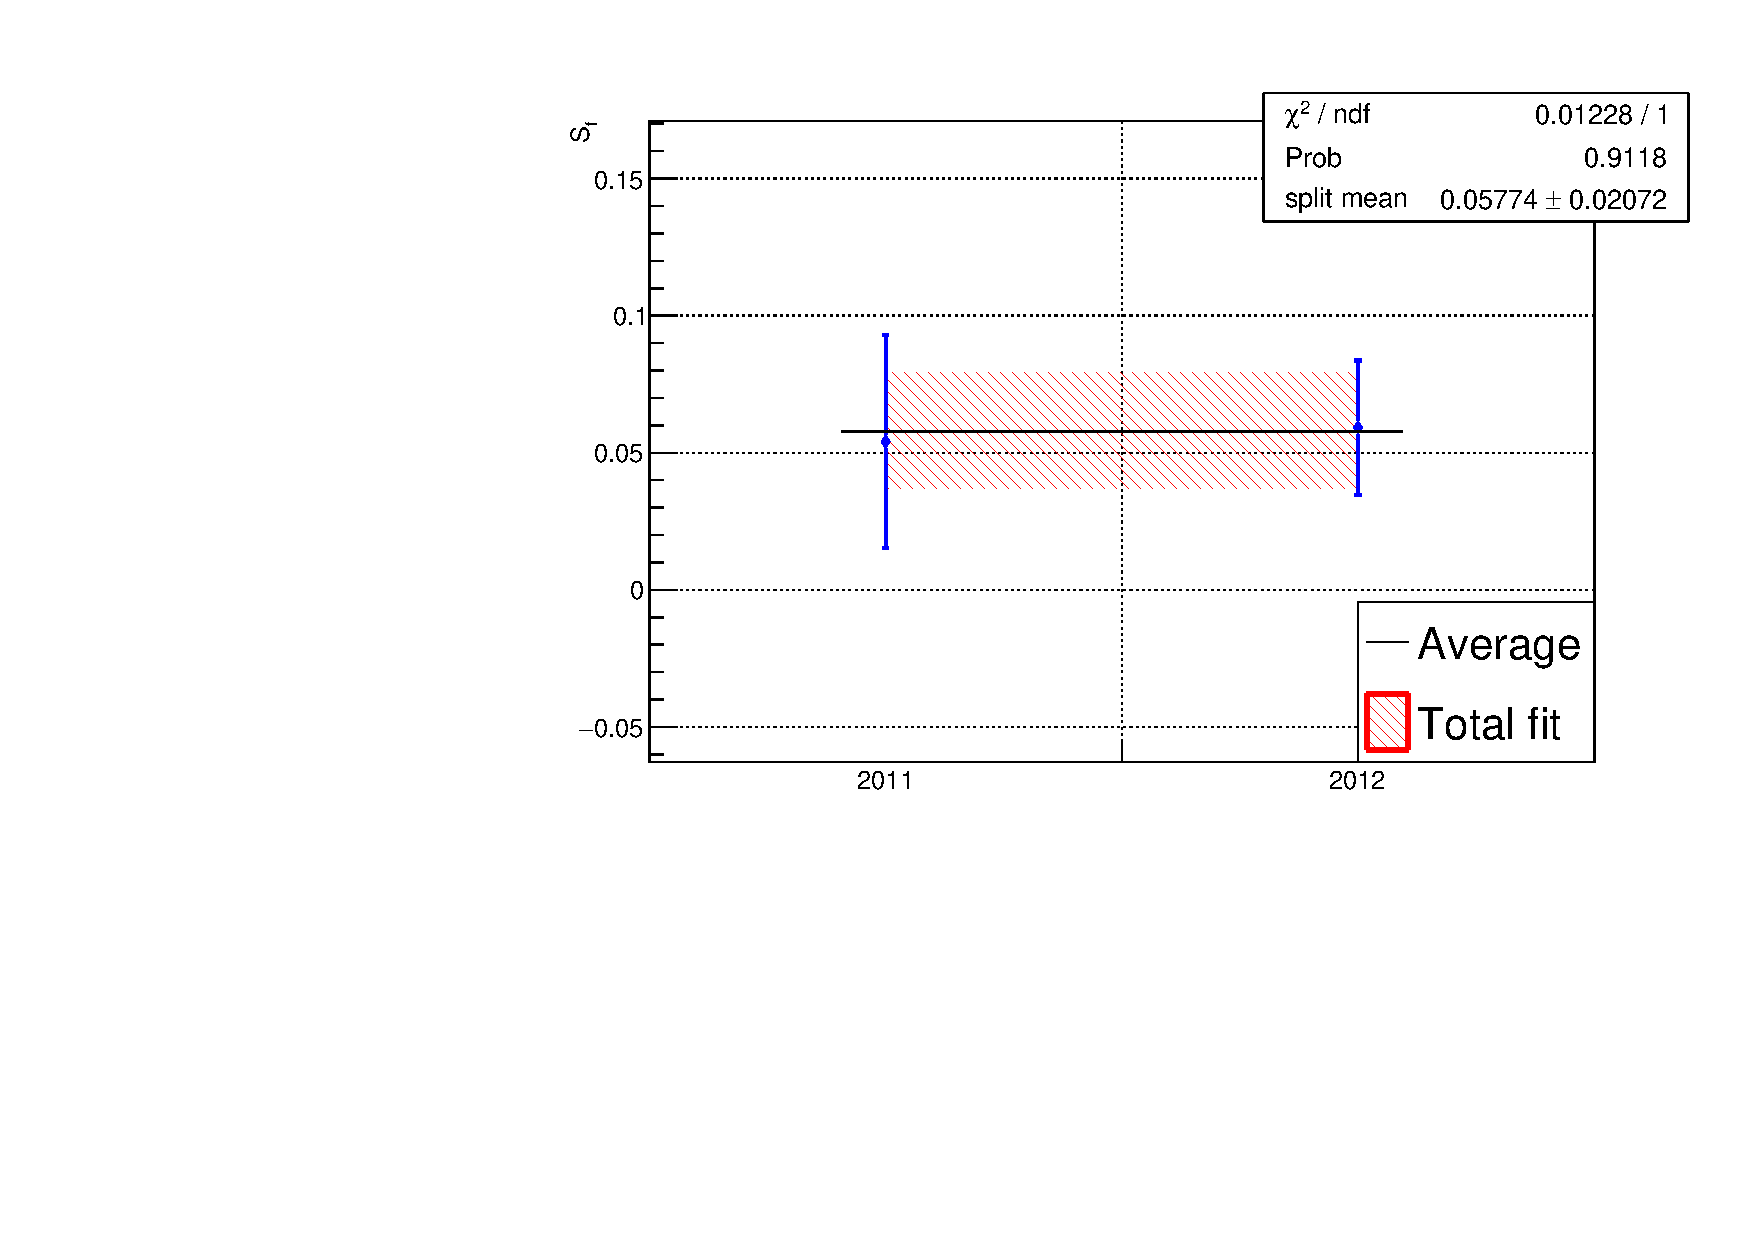
\includegraphics[width=0.49\textwidth]{05DecaytimeFit/figs/splits/Sf_splits_Year.pdf}
    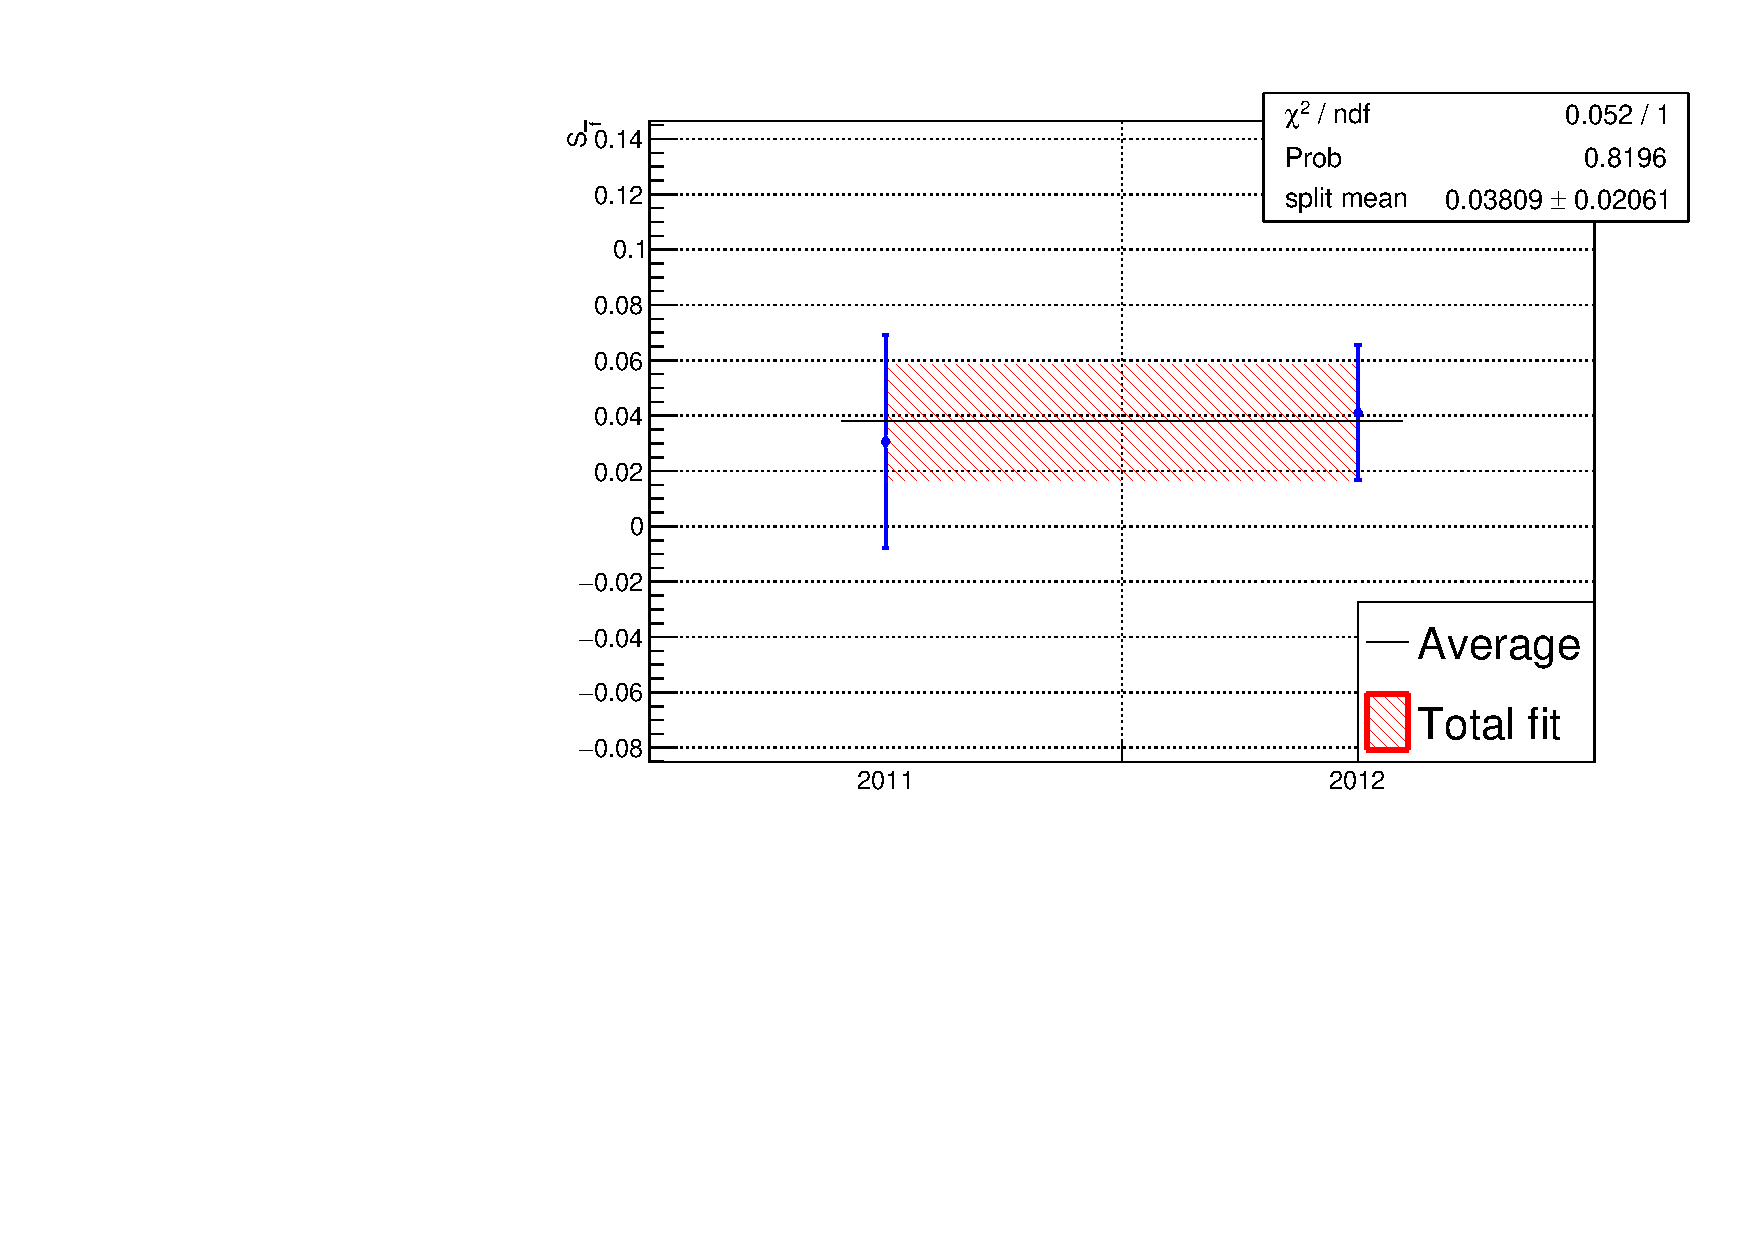
\includegraphics[width=0.49\textwidth]{05DecaytimeFit/figs/splits/Sfbar_splits_Year.pdf} \\
    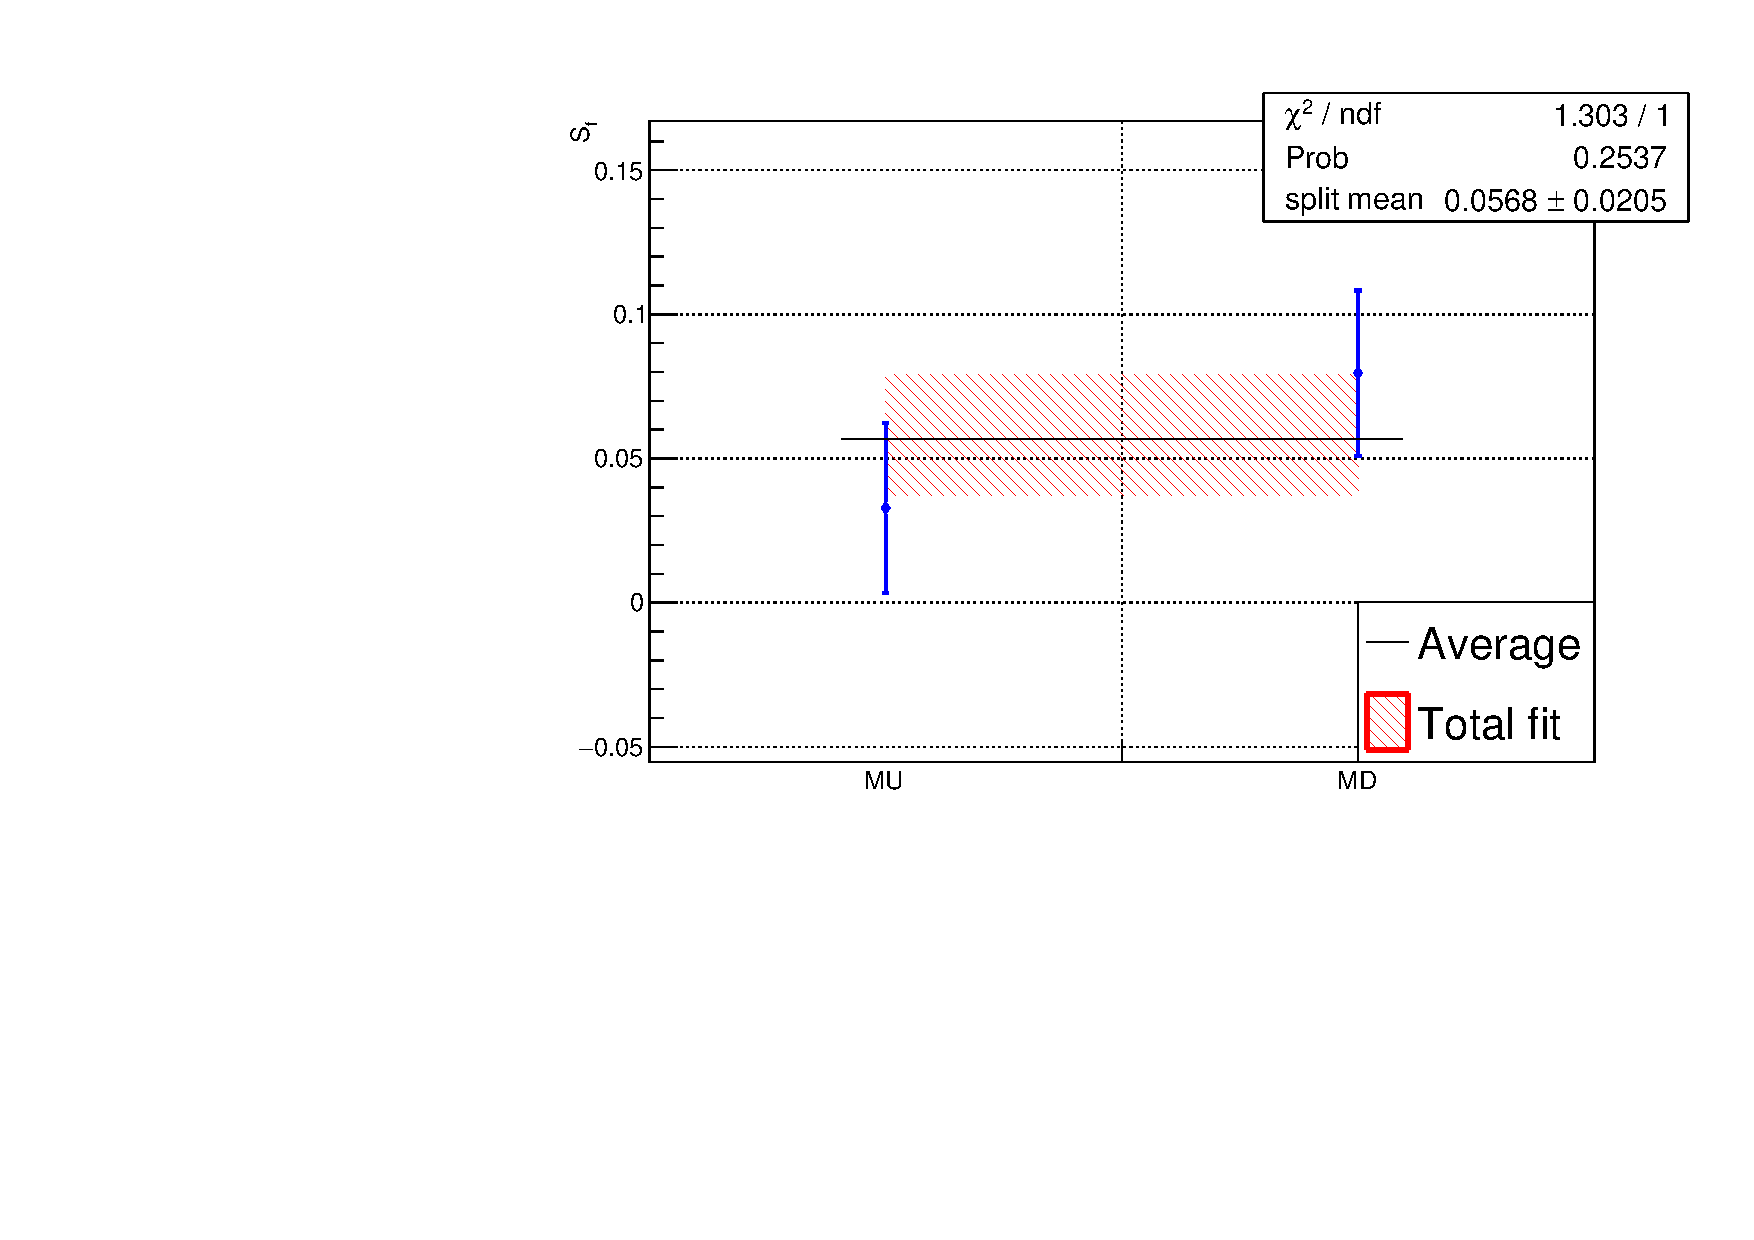
\includegraphics[width=0.49\textwidth]{05DecaytimeFit/figs/splits/Sf_splits_Polarity.pdf}
    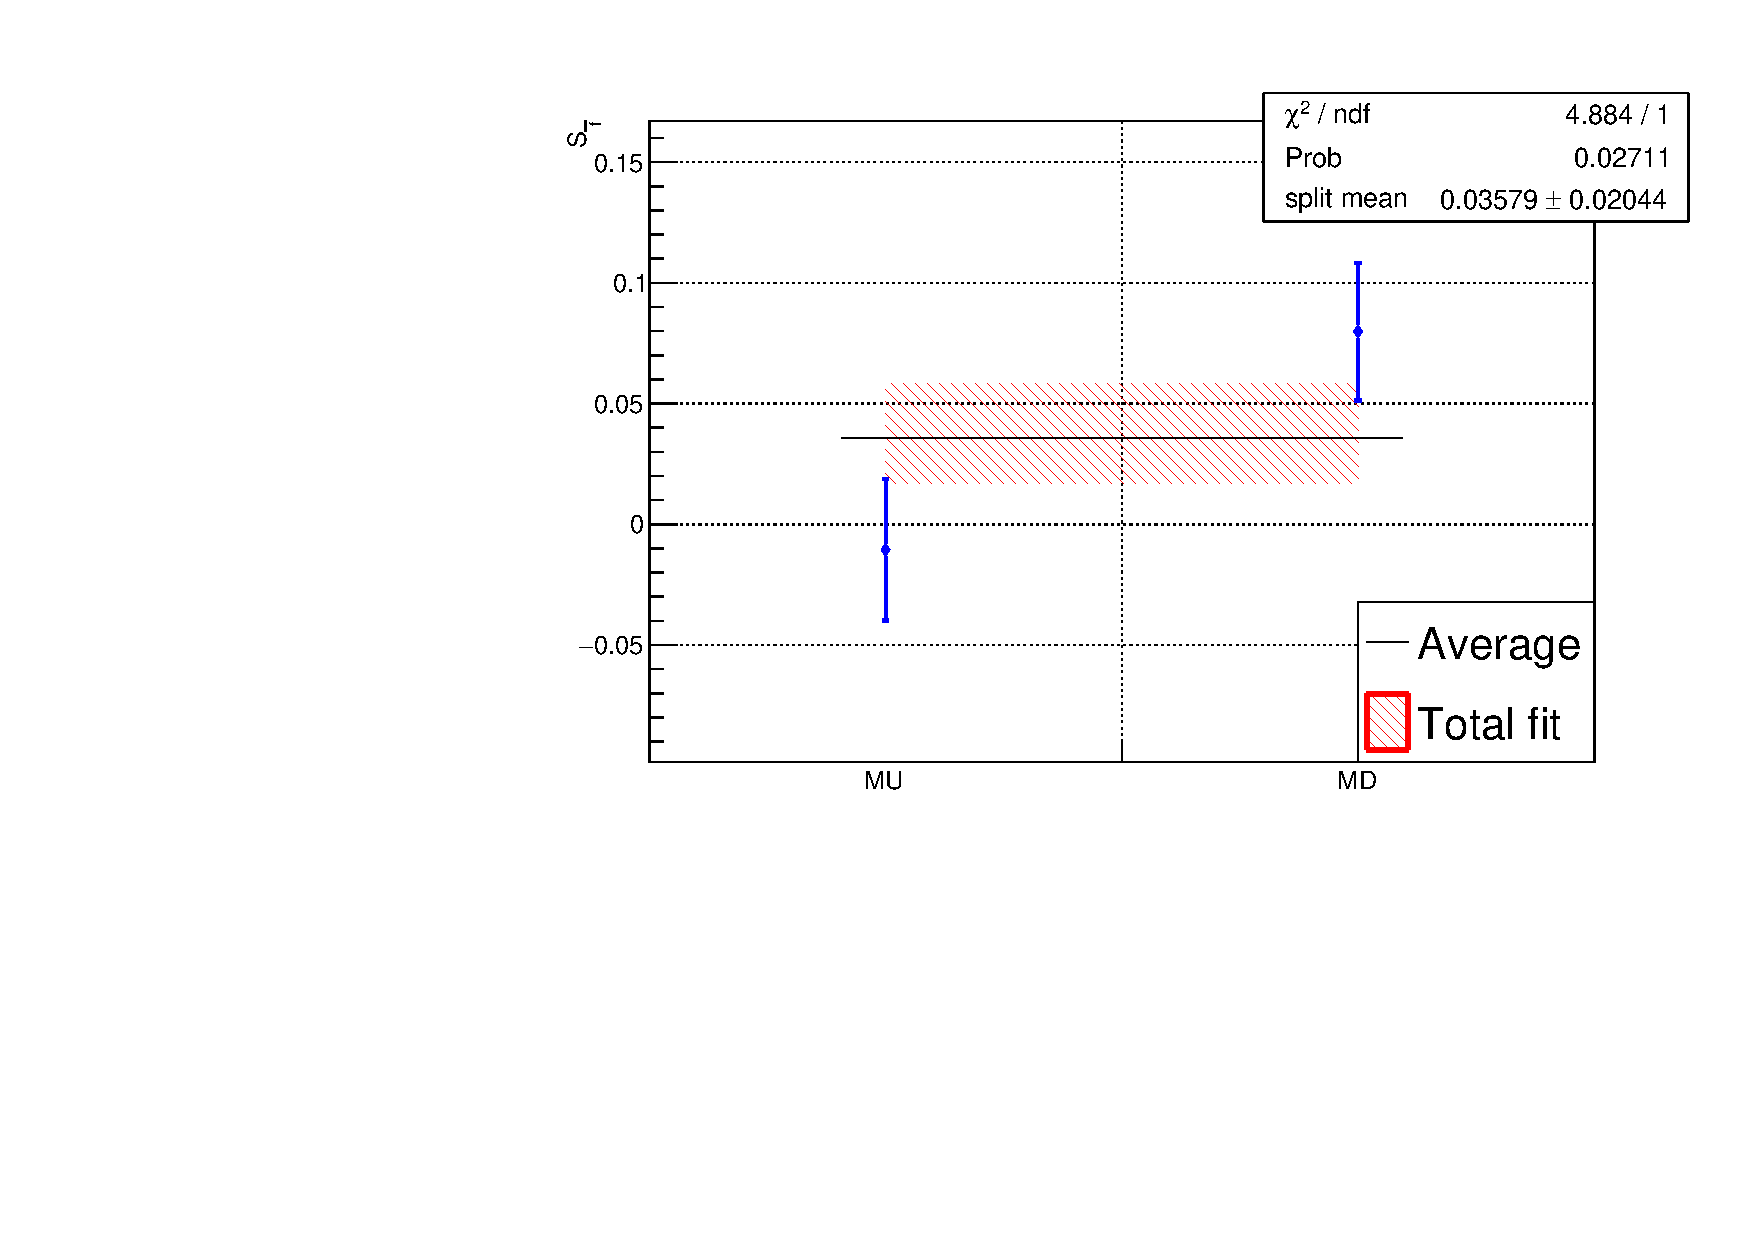
\includegraphics[width=0.49\textwidth]{05DecaytimeFit/figs/splits/Sfbar_splits_Polarity.pdf}
    \end{center}
  \vspace{-2mm}
  \caption{Fitted values of $S_f$ (left) and $S_{\bar f}$ (right) as a function of the data-taking year (top) and magnet polarity
  (bottom). The red hatched band shows the values obtained from the nominal fit of the full sample.
  The horizontal black line is the result of a $\chi^2$ fit to obtain the weighted average of the results of each subsample.}
  \label{fig:year_pol_splits}
\end{figure}

The stability of the results against the tagging algorithm adopted in the fit are also checked. In this case, the data
sample with \emph{sWeights} obtained from the nominal mass fit (Sec.~\ref{sec:massfit}) is split in three independent subsamples
according to the tagging decision:
\begin{itemize}[noitemsep,topsep=0pt]
  \item candidates tagged exclusively by the OS tagger;
  \item candidates tagged exclusively by the SS tagger;
  \item candidates tagged by both the OS and SS taggers.
\end{itemize}
The values of $S_{f}$ and  $S_{\bar{f}}$ obtained in these subsamples are compared in Fig.~\ref{fig:tagging_splits}.
All values are compatible. More details are given in Appendix~\ref{app:timesplits}. Given the
difference of the tagging algorithms and their calibrations, the stability of the results in this test provides additional
confidence on the strategy adopted of floating the calibration parameters in the fit.

\begin{figure}[htpb]
        \begin{center}
                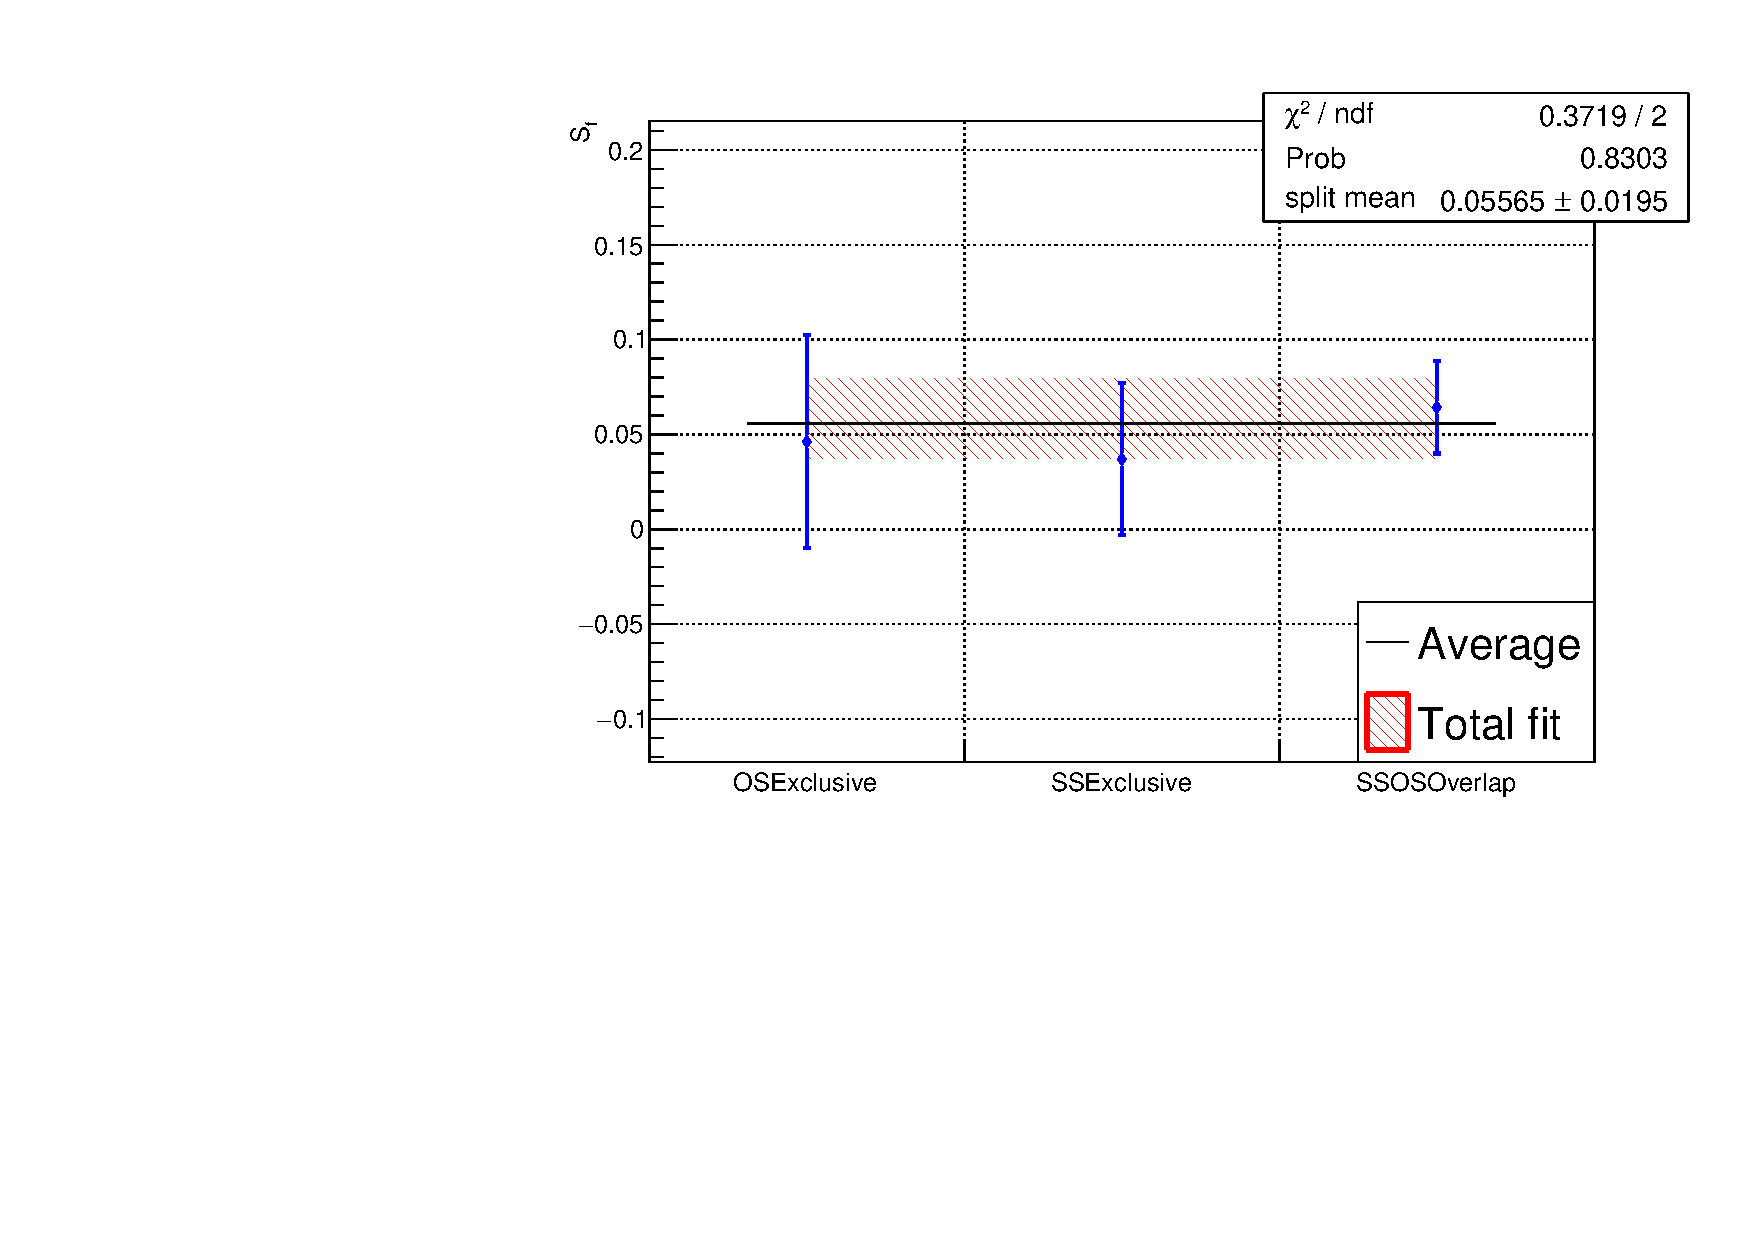
\includegraphics[width=0.49\textwidth]{05DecaytimeFit/figs/splits/Sf_splits_SSOSExclusive.pdf}
                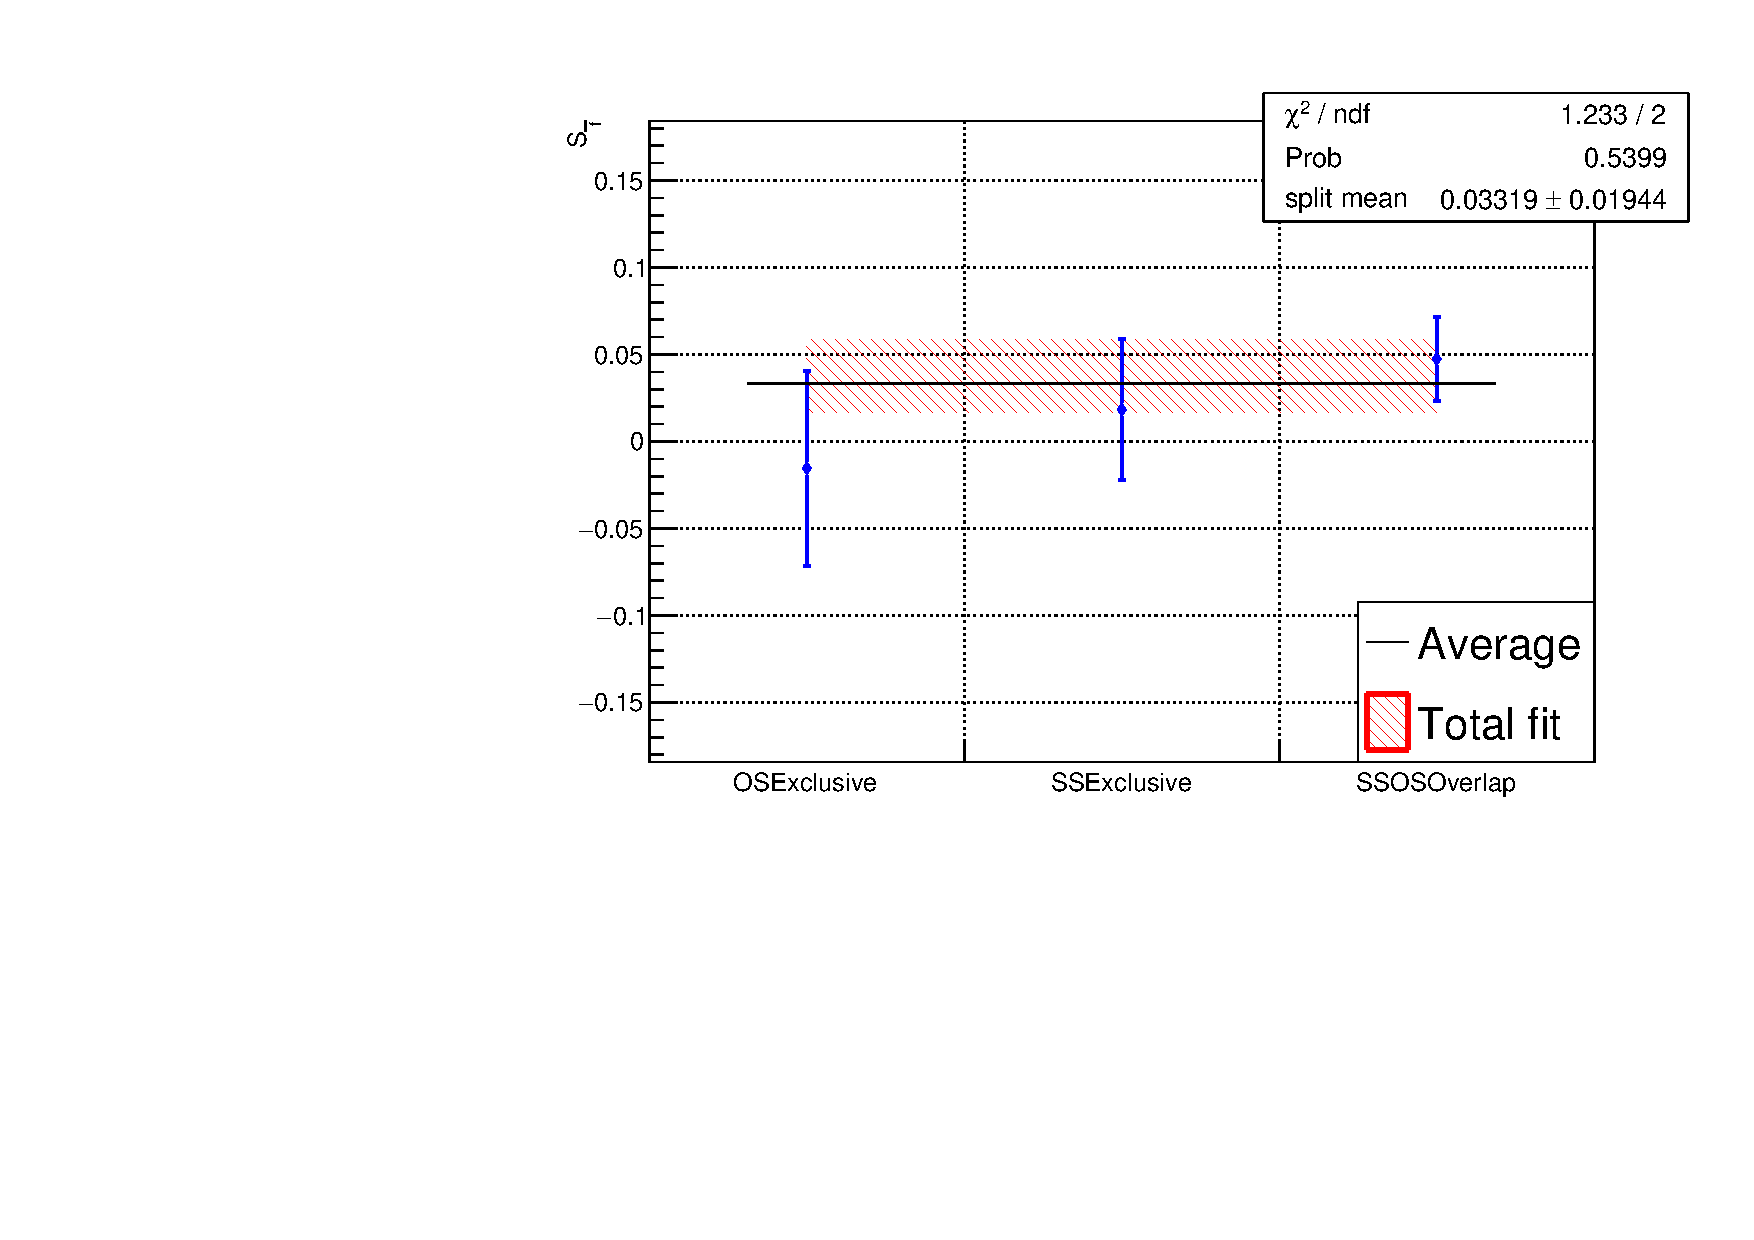
\includegraphics[width=0.49\textwidth]{05DecaytimeFit/figs/splits/Sfbar_splits_SSOSExclusive.pdf}
        \end{center}
        \vspace{-2mm}
        \caption{Fitted values of $S_f$ (left) and $S_{\bar f}$ (right) when candidates tagged
        exclusively by OS or SS, or both simultaneously are considered. 
        The red hatched band shows the values obtained from the nominal fit of the full sample.
        The horizontal black line is the result of a $\chi^2$ fit to obtain the weighted average of the results of each subsample.}
        \label{fig:tagging_splits}
\end{figure}

The stability of the results against the $\Bz$ kinematics and global properties of the event is tested.
More specifically, the decay time fit is repeated in bins of the following variables:
\begin{itemize}[noitemsep,topsep=0pt]
  \item transverse momentum of the $\Bz$ (4 bins);
  \item number of reconstructed primary vertices (3 bins);
  \item total number of reconstructed tracks (3 bins);
  \item difference in pseudorapidity ($\Delta\eta$) between $D$ meson and bachelor pion (4 bins).
\end{itemize}
The motivation for these tests is that flavour tagging calibration parameters depend on the above observables; as a consequence, the
fitted values for the $S_f$ and $S_{\bar f}$ coefficients might also show a significant trend in these variables because of
the correlation with the flavour tagging calibrations.
Moreover, the difference is pseudorapidity is sensitive to potential misalignments in the detectors which might affect the measured value of \CP~asymmetries.
The values of $S_{f}$ and  $S_{\bar{f}}$ obtained in these subsamples are compared in Fig.~\ref{fig:kin_evt_splits}, whereas more
details are given in Appendix~\ref{app:timesplits}.
All values are compatible, and no significant dependence of $S_f$ and $S_{\bar f}$ on the studied variables is observed.
\begin{figure}[htpb]
        \begin{center}
                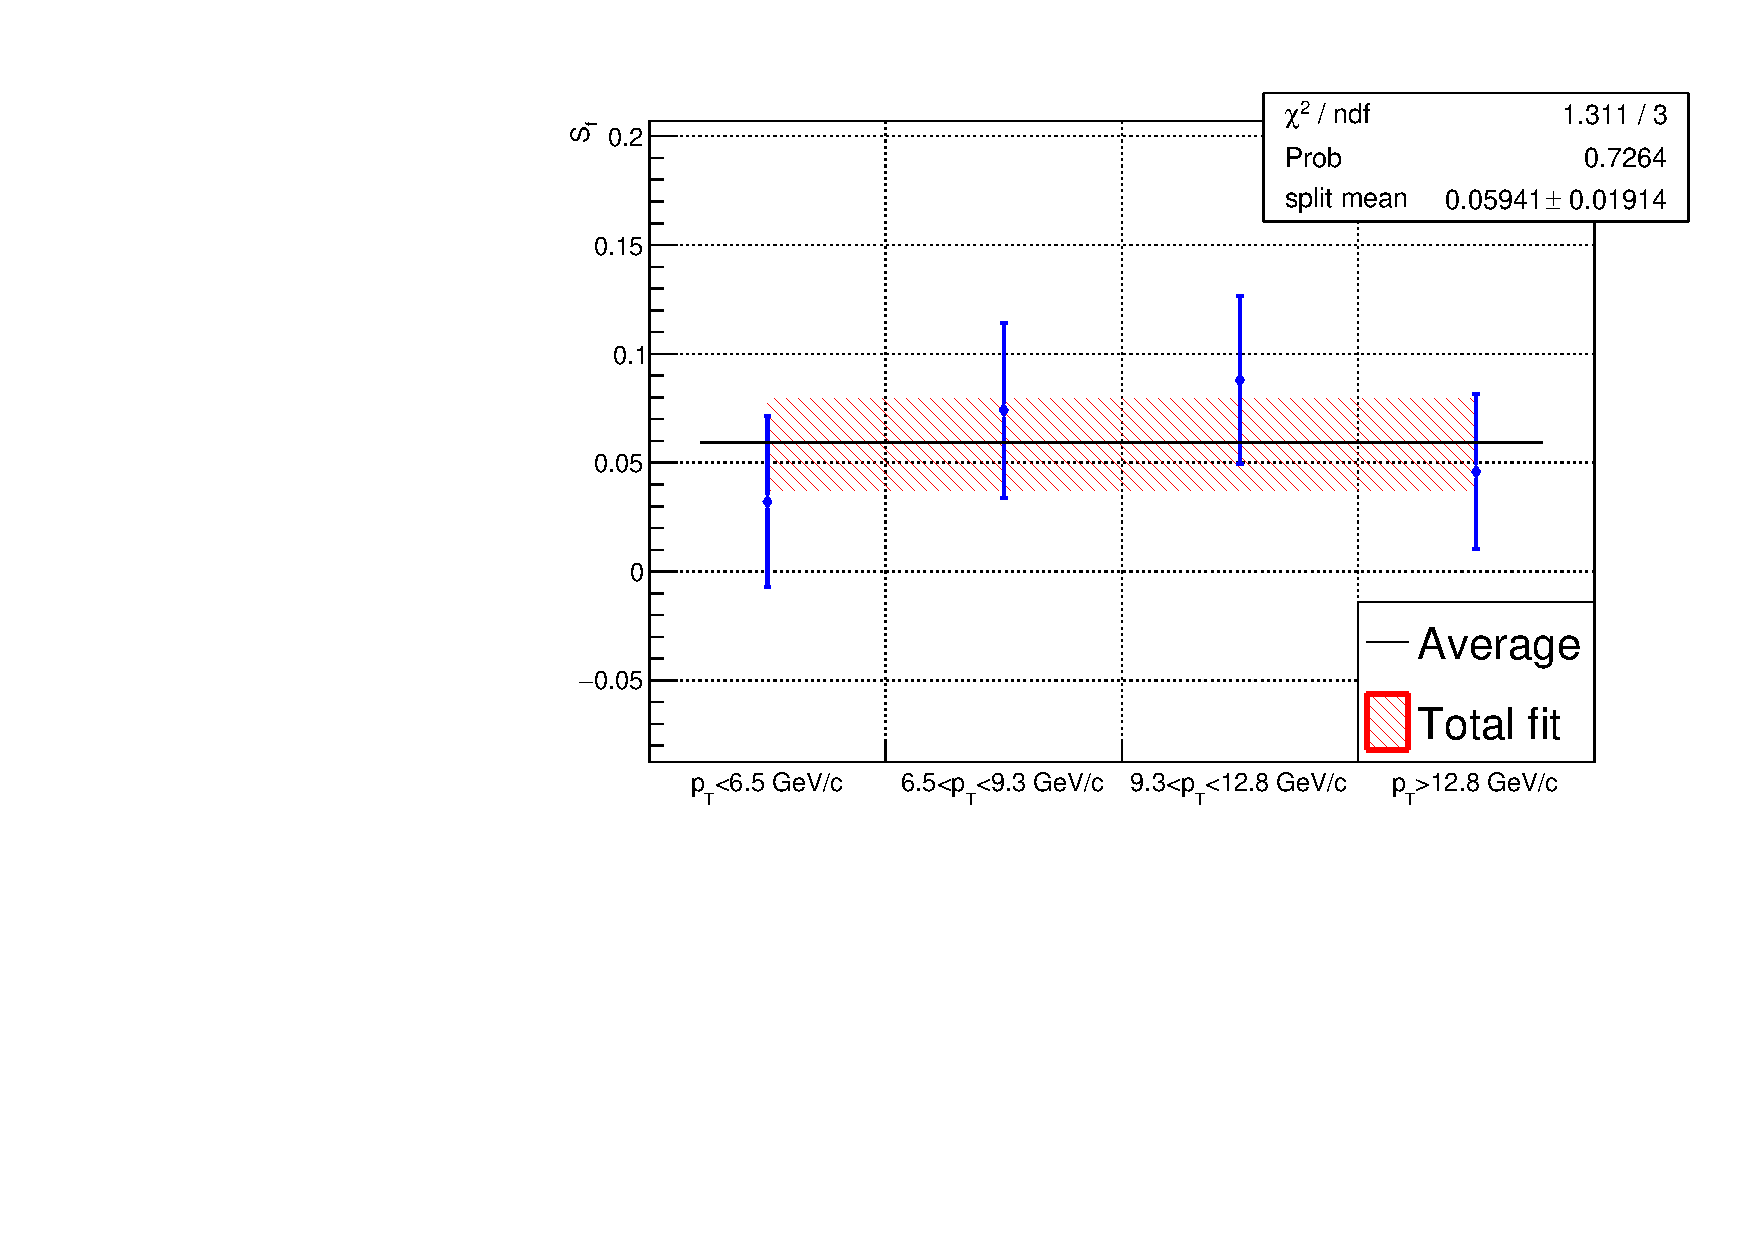
\includegraphics[width=0.45\textwidth]{05DecaytimeFit/figs/splits/Sf_splits_BPT.pdf}
                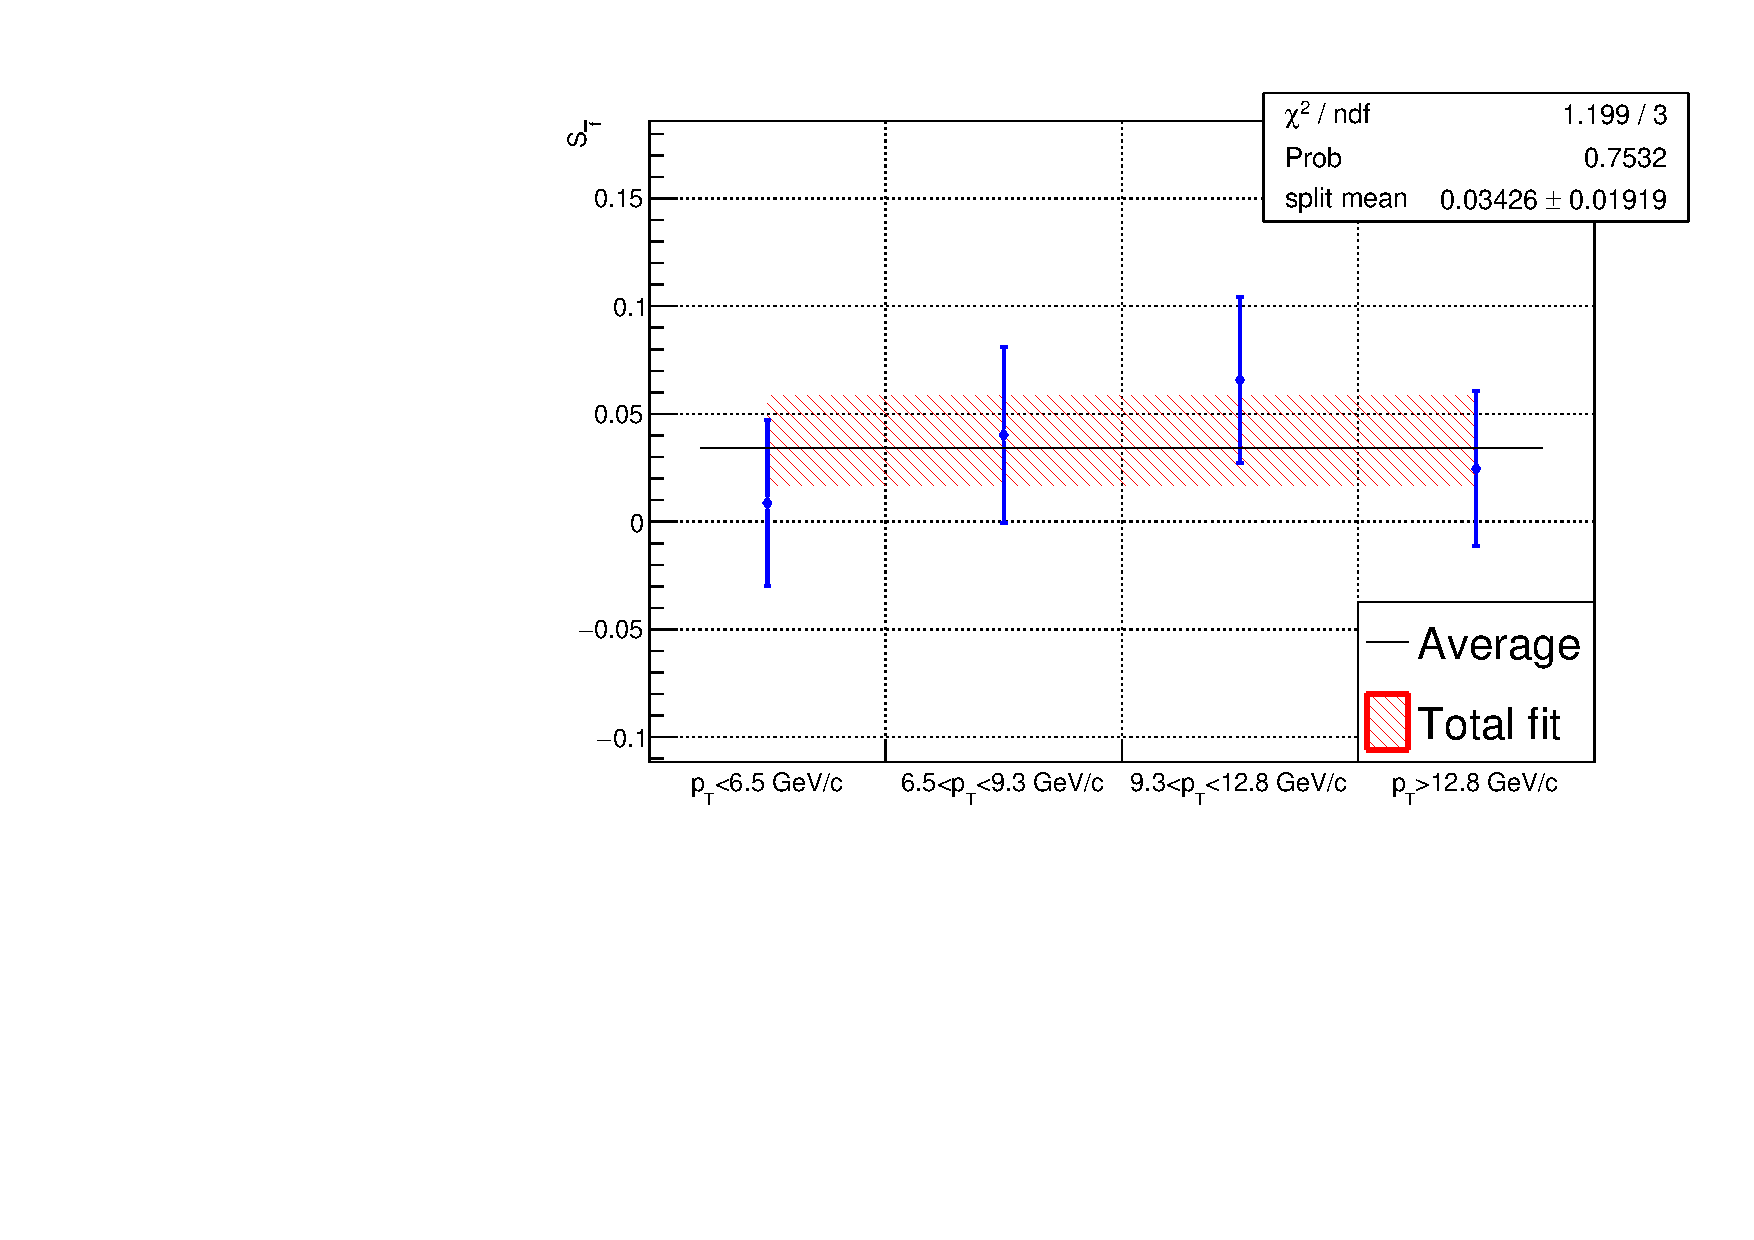
\includegraphics[width=0.45\textwidth]{05DecaytimeFit/figs/splits/Sfbar_splits_BPT.pdf} \\
                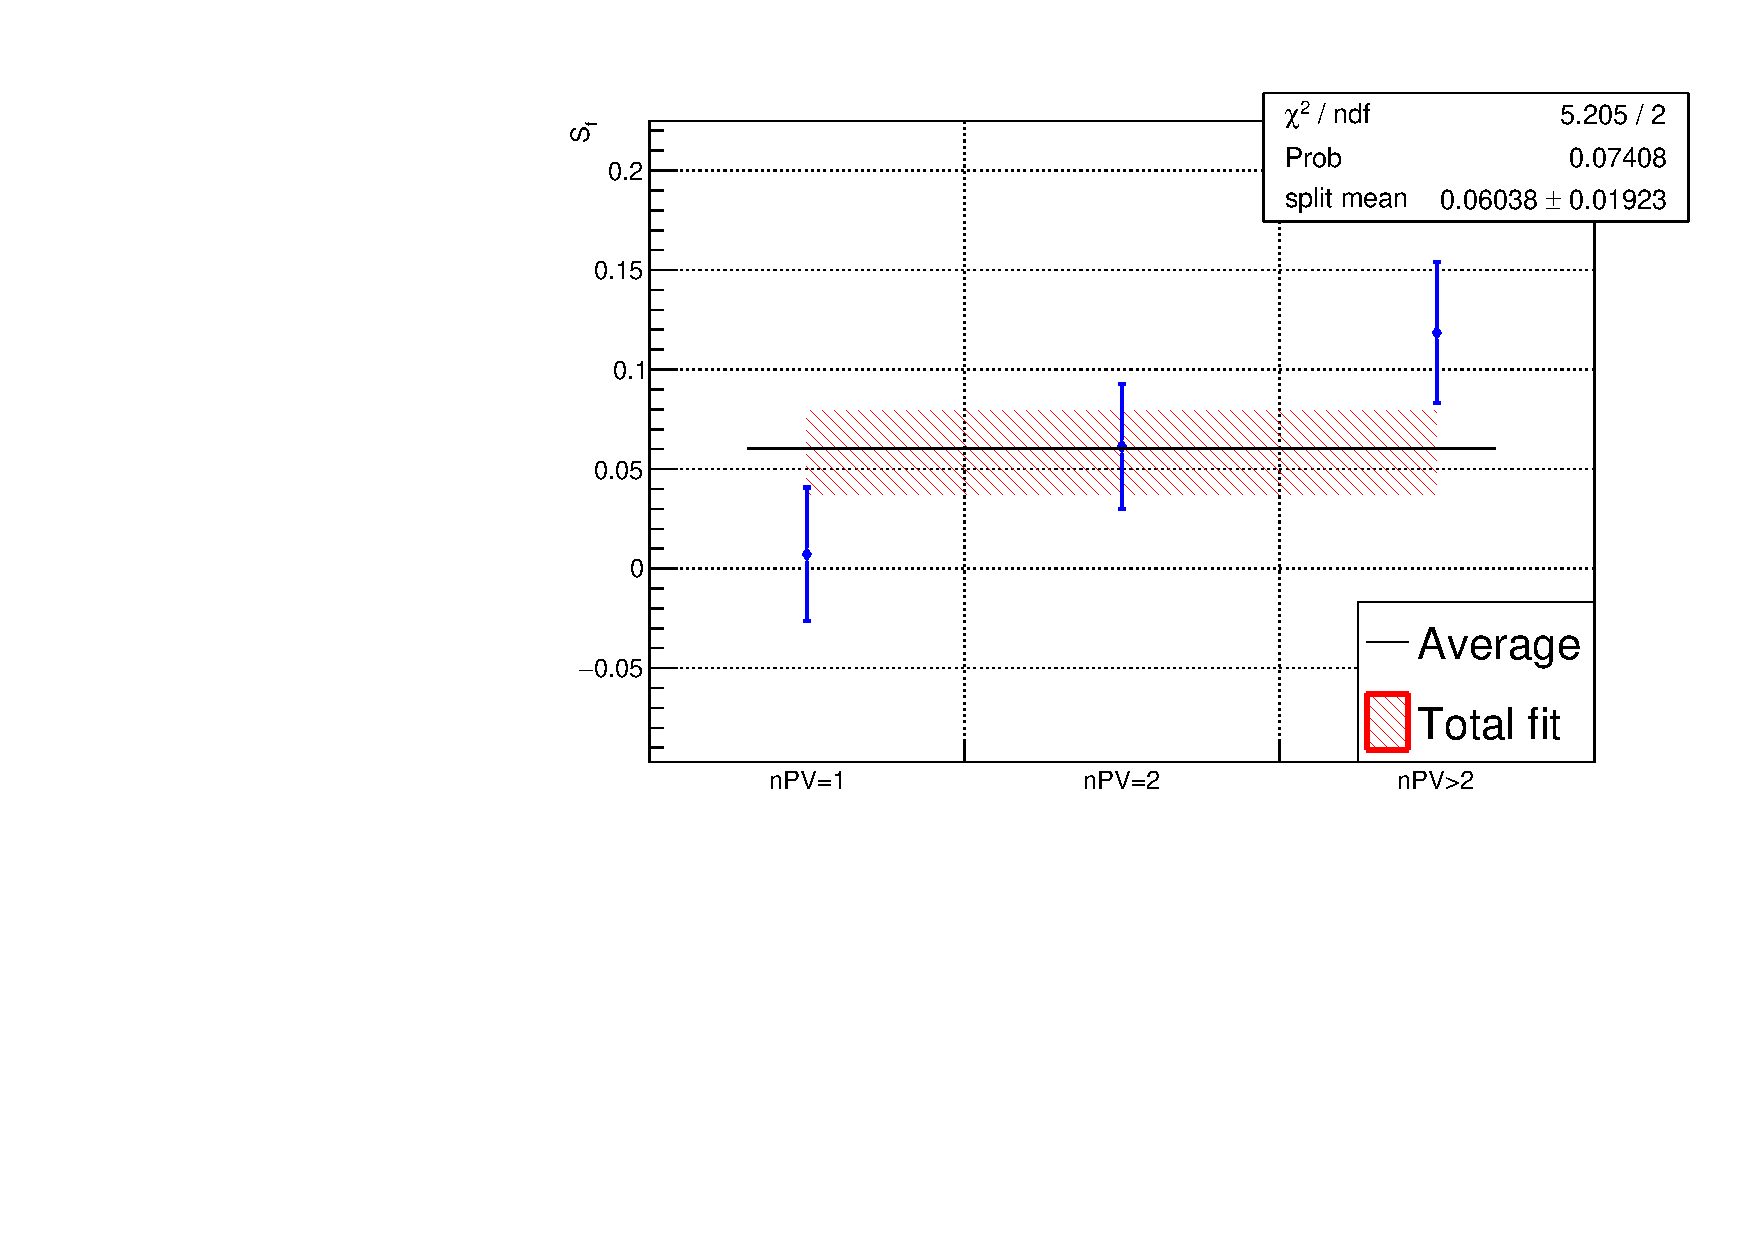
\includegraphics[width=0.45\textwidth]{05DecaytimeFit/figs/splits/Sf_splits_nPV.pdf}
                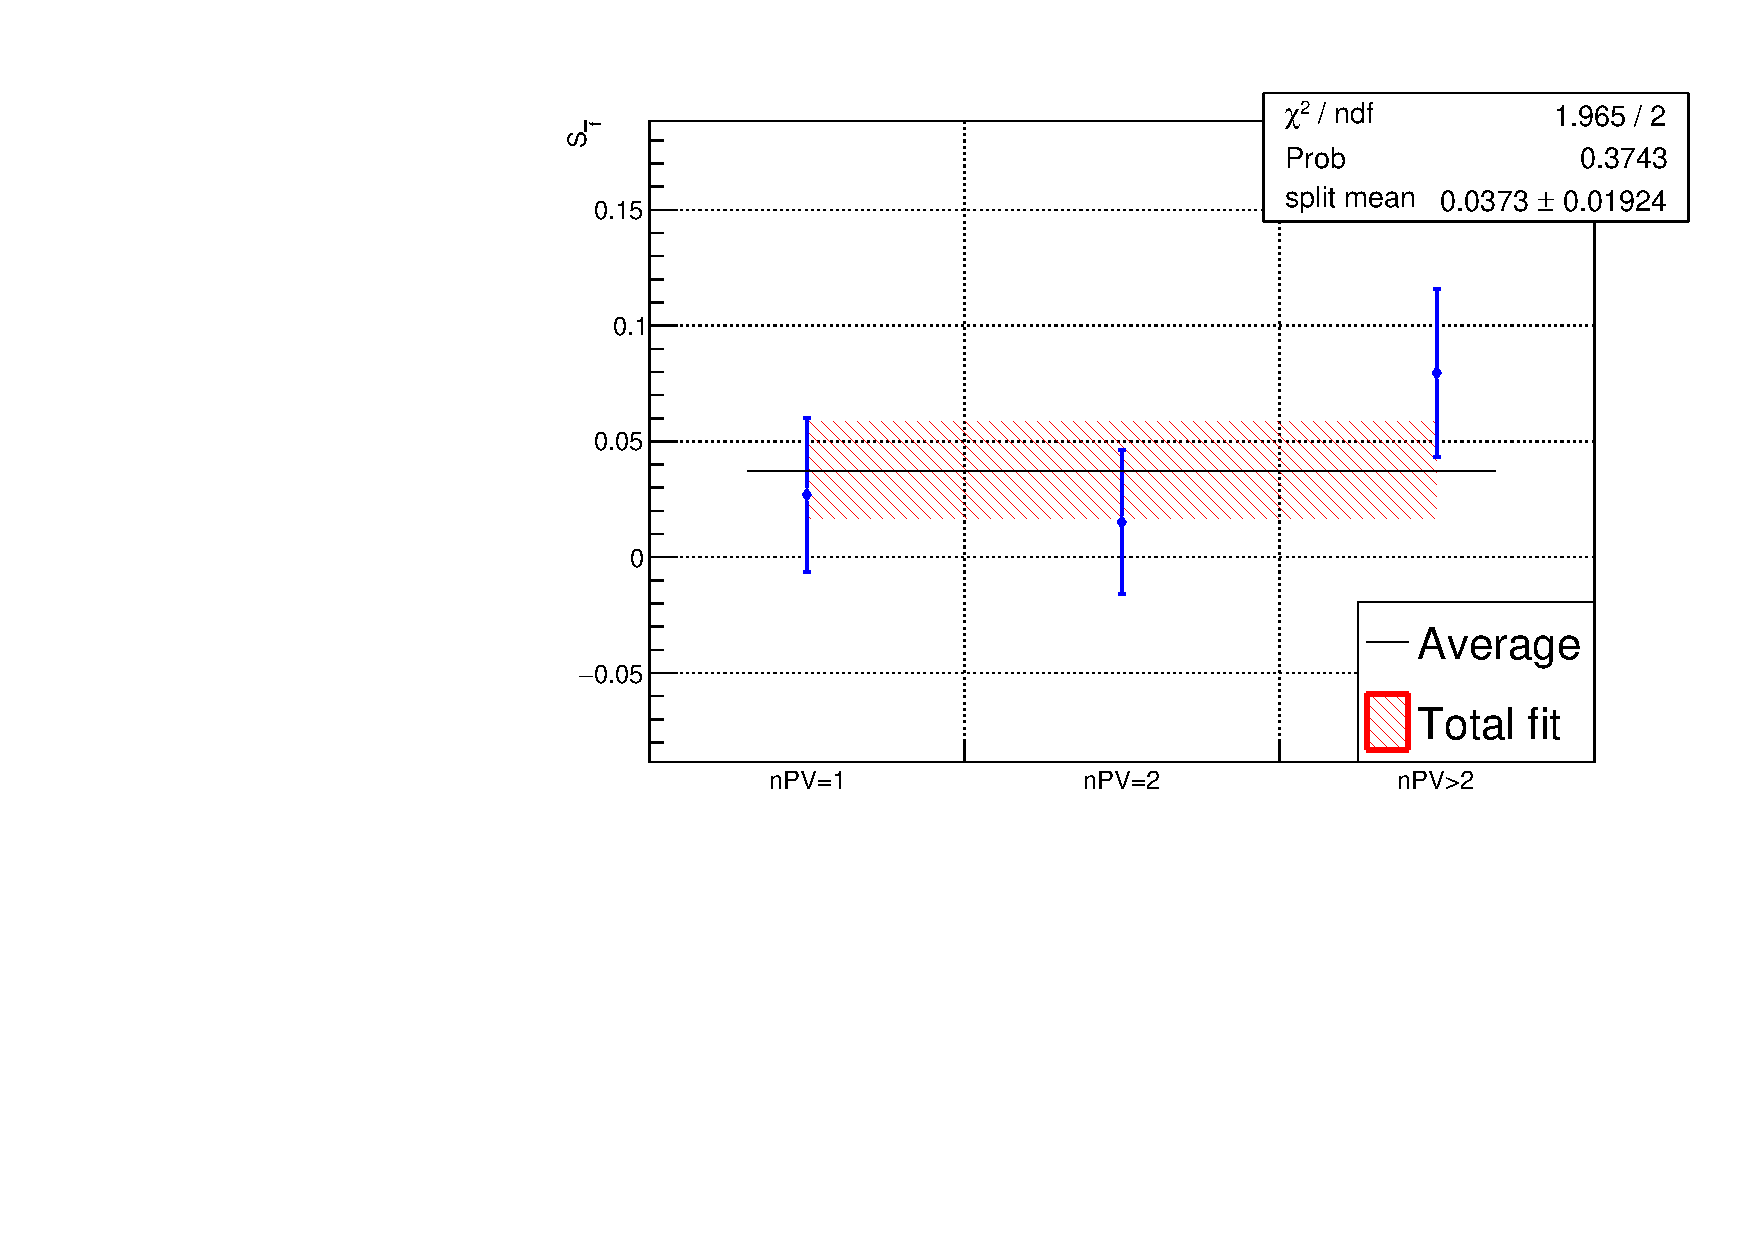
\includegraphics[width=0.45\textwidth]{05DecaytimeFit/figs/splits/Sfbar_splits_nPV.pdf} \\
                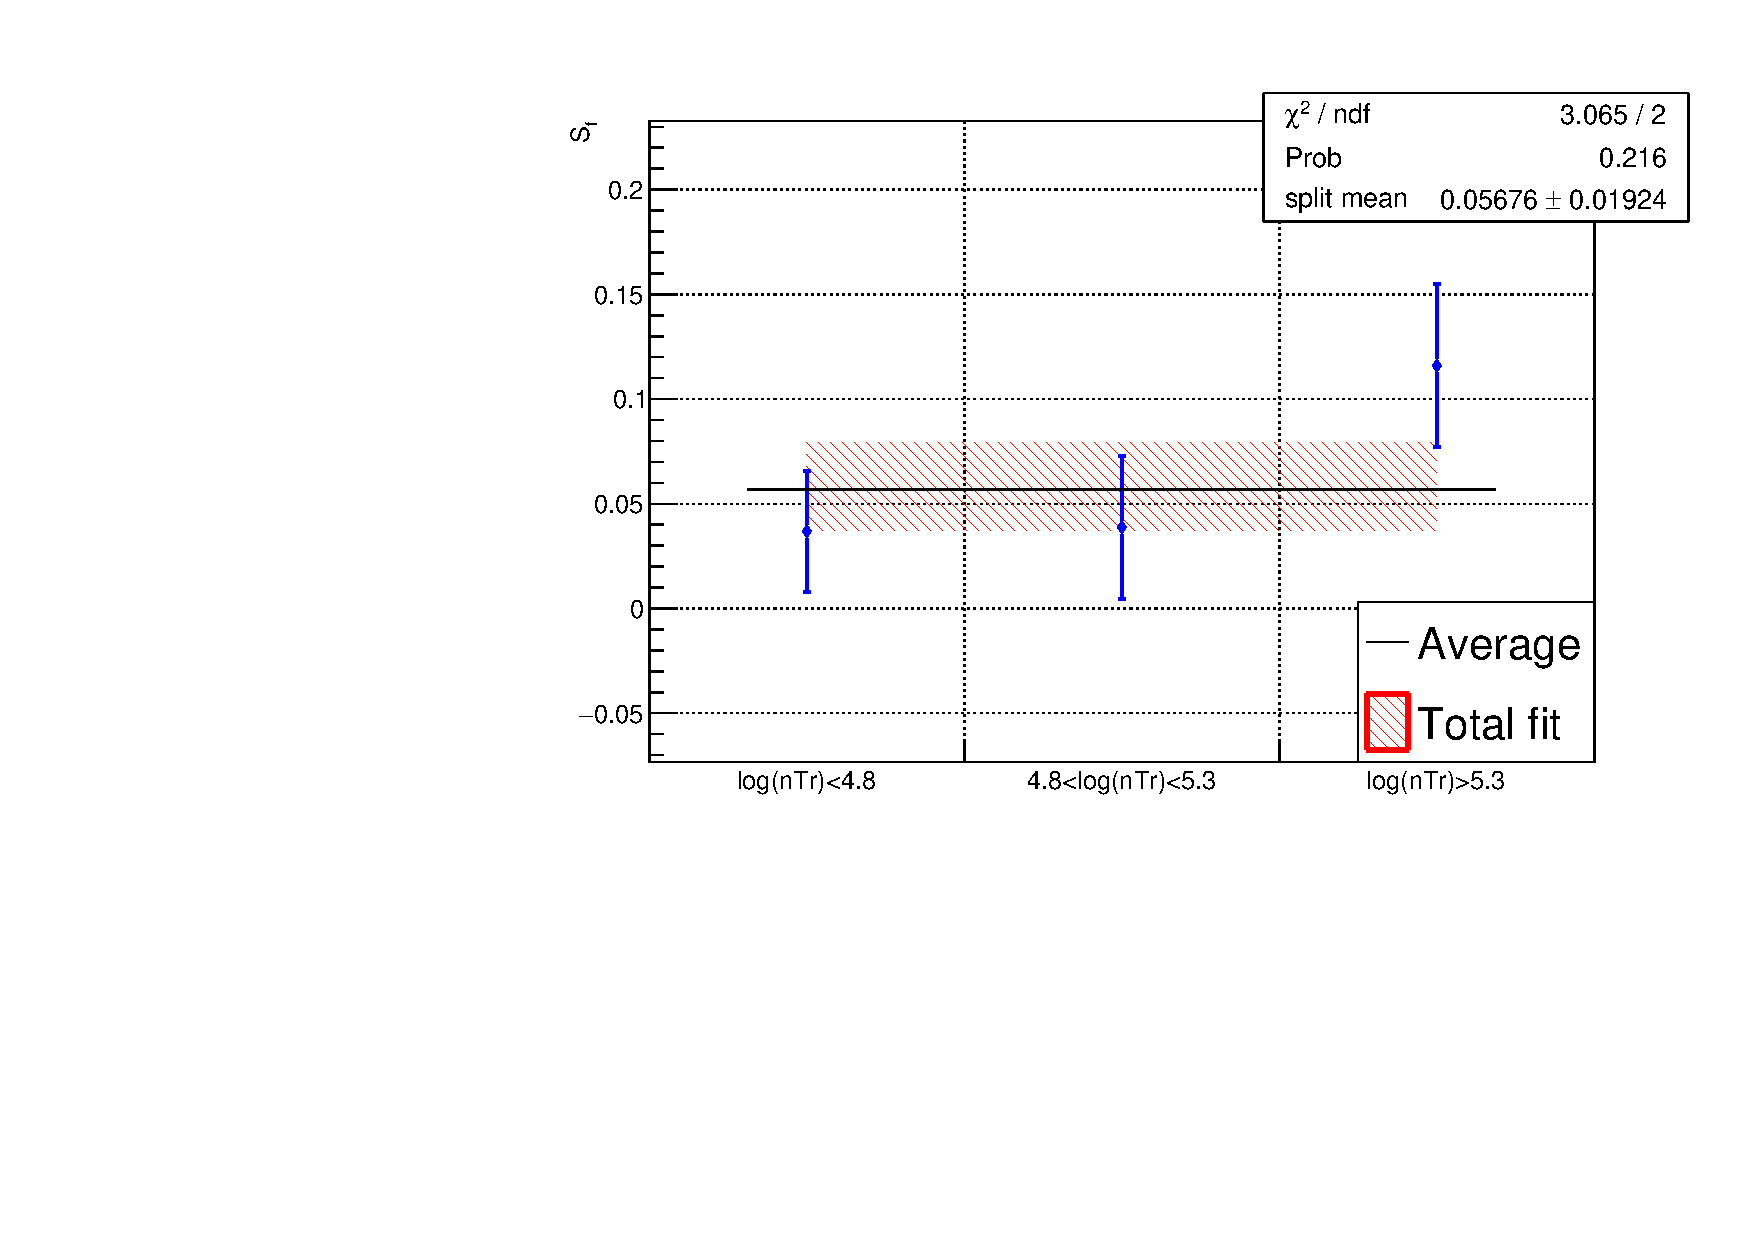
\includegraphics[width=0.45\textwidth]{05DecaytimeFit/figs/splits/Sf_splits_nTracks.pdf}
                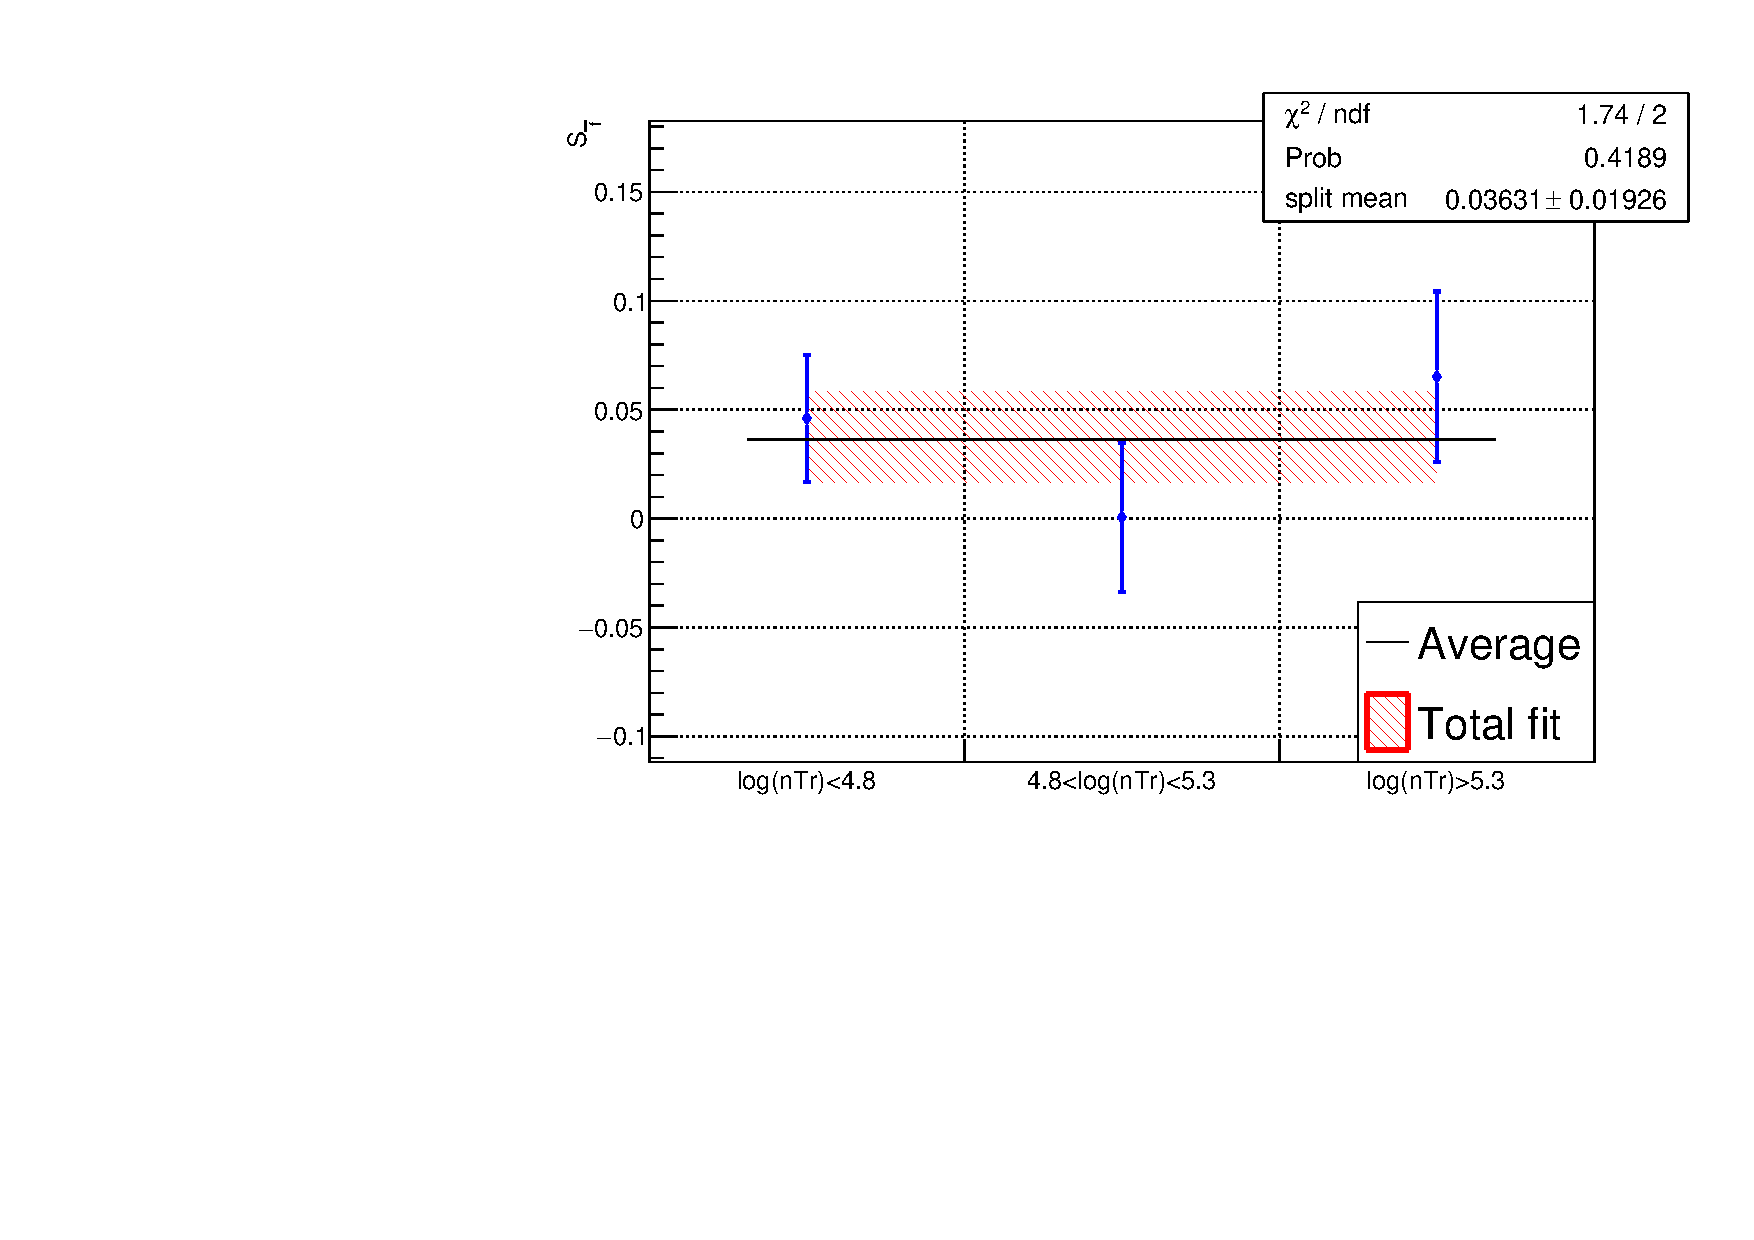
\includegraphics[width=0.45\textwidth]{05DecaytimeFit/figs/splits/Sfbar_splits_nTracks.pdf} \\
                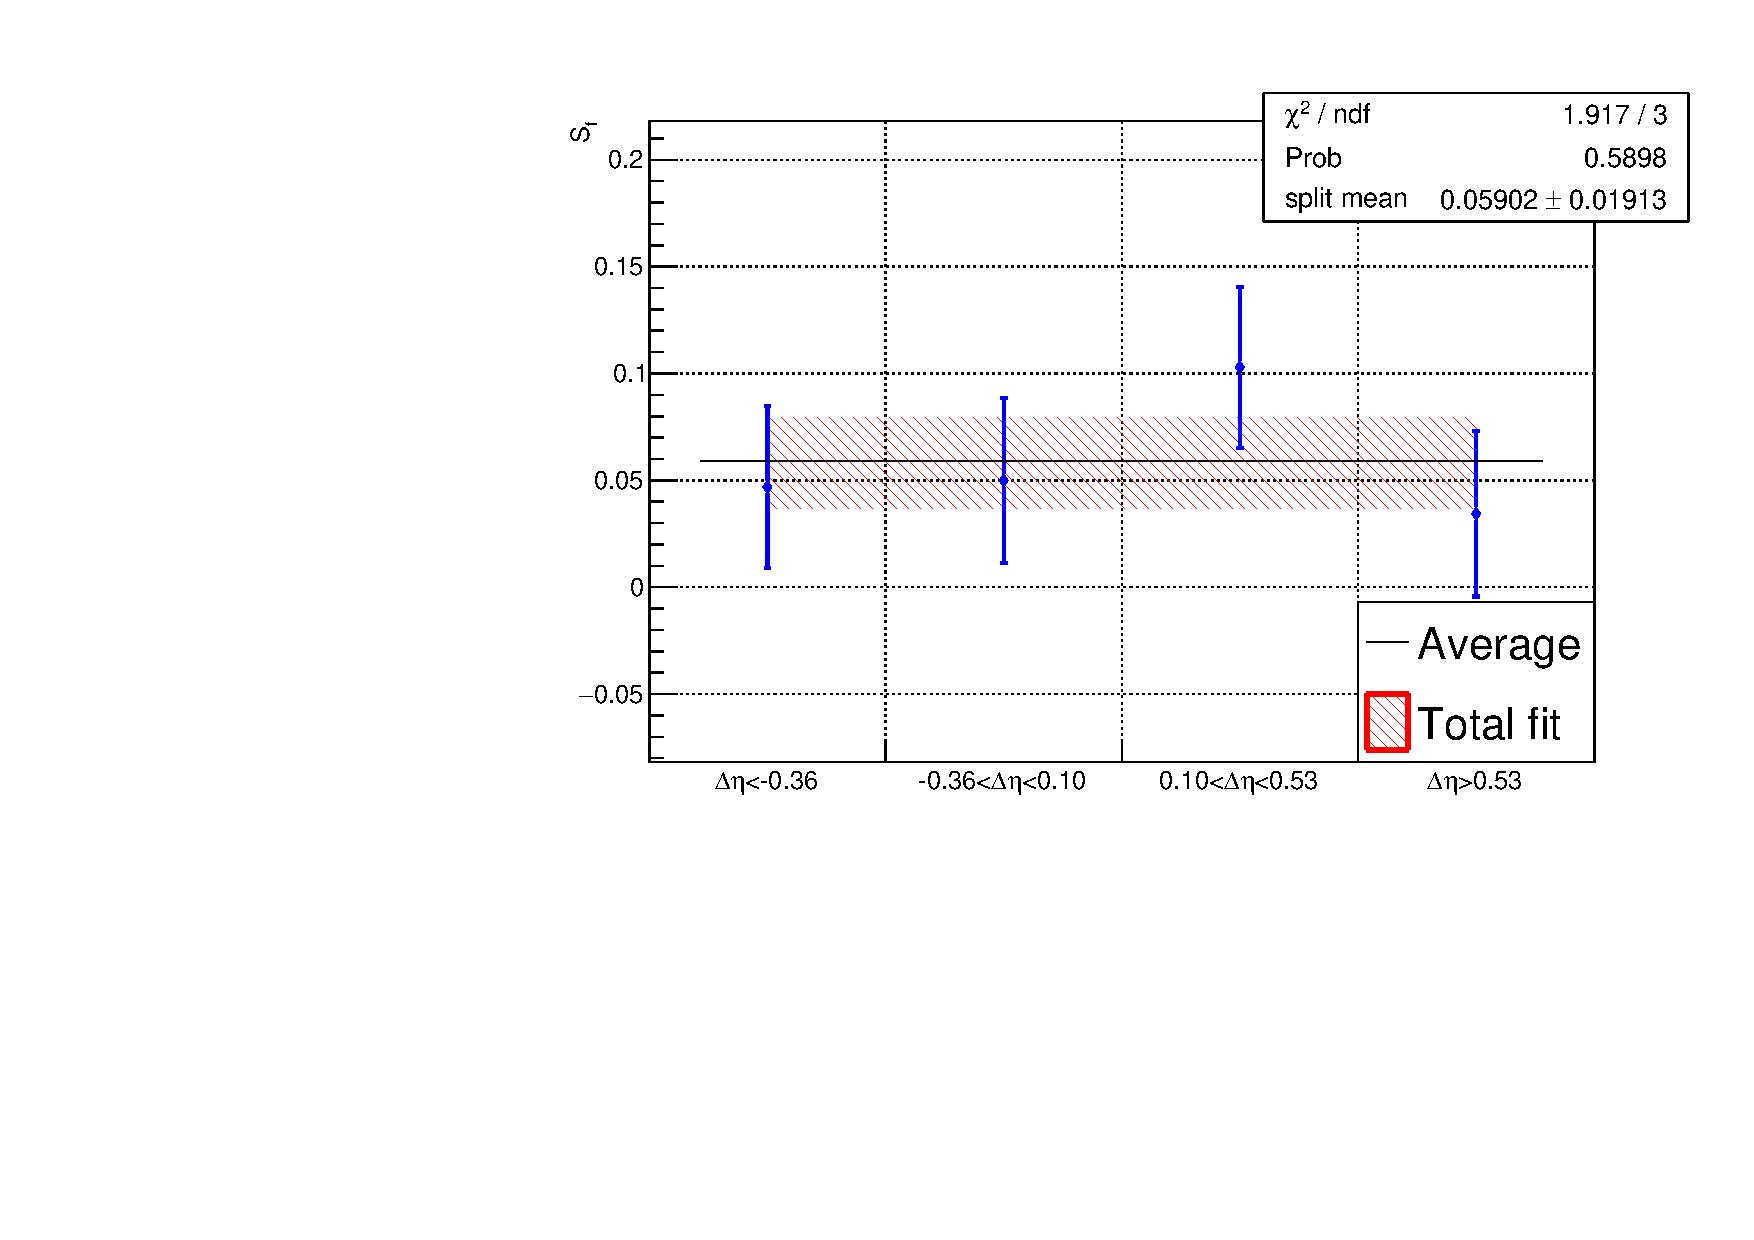
\includegraphics[width=0.45\textwidth]{05DecaytimeFit/figs/splits/Sf_splits_DeltaEta.pdf}
                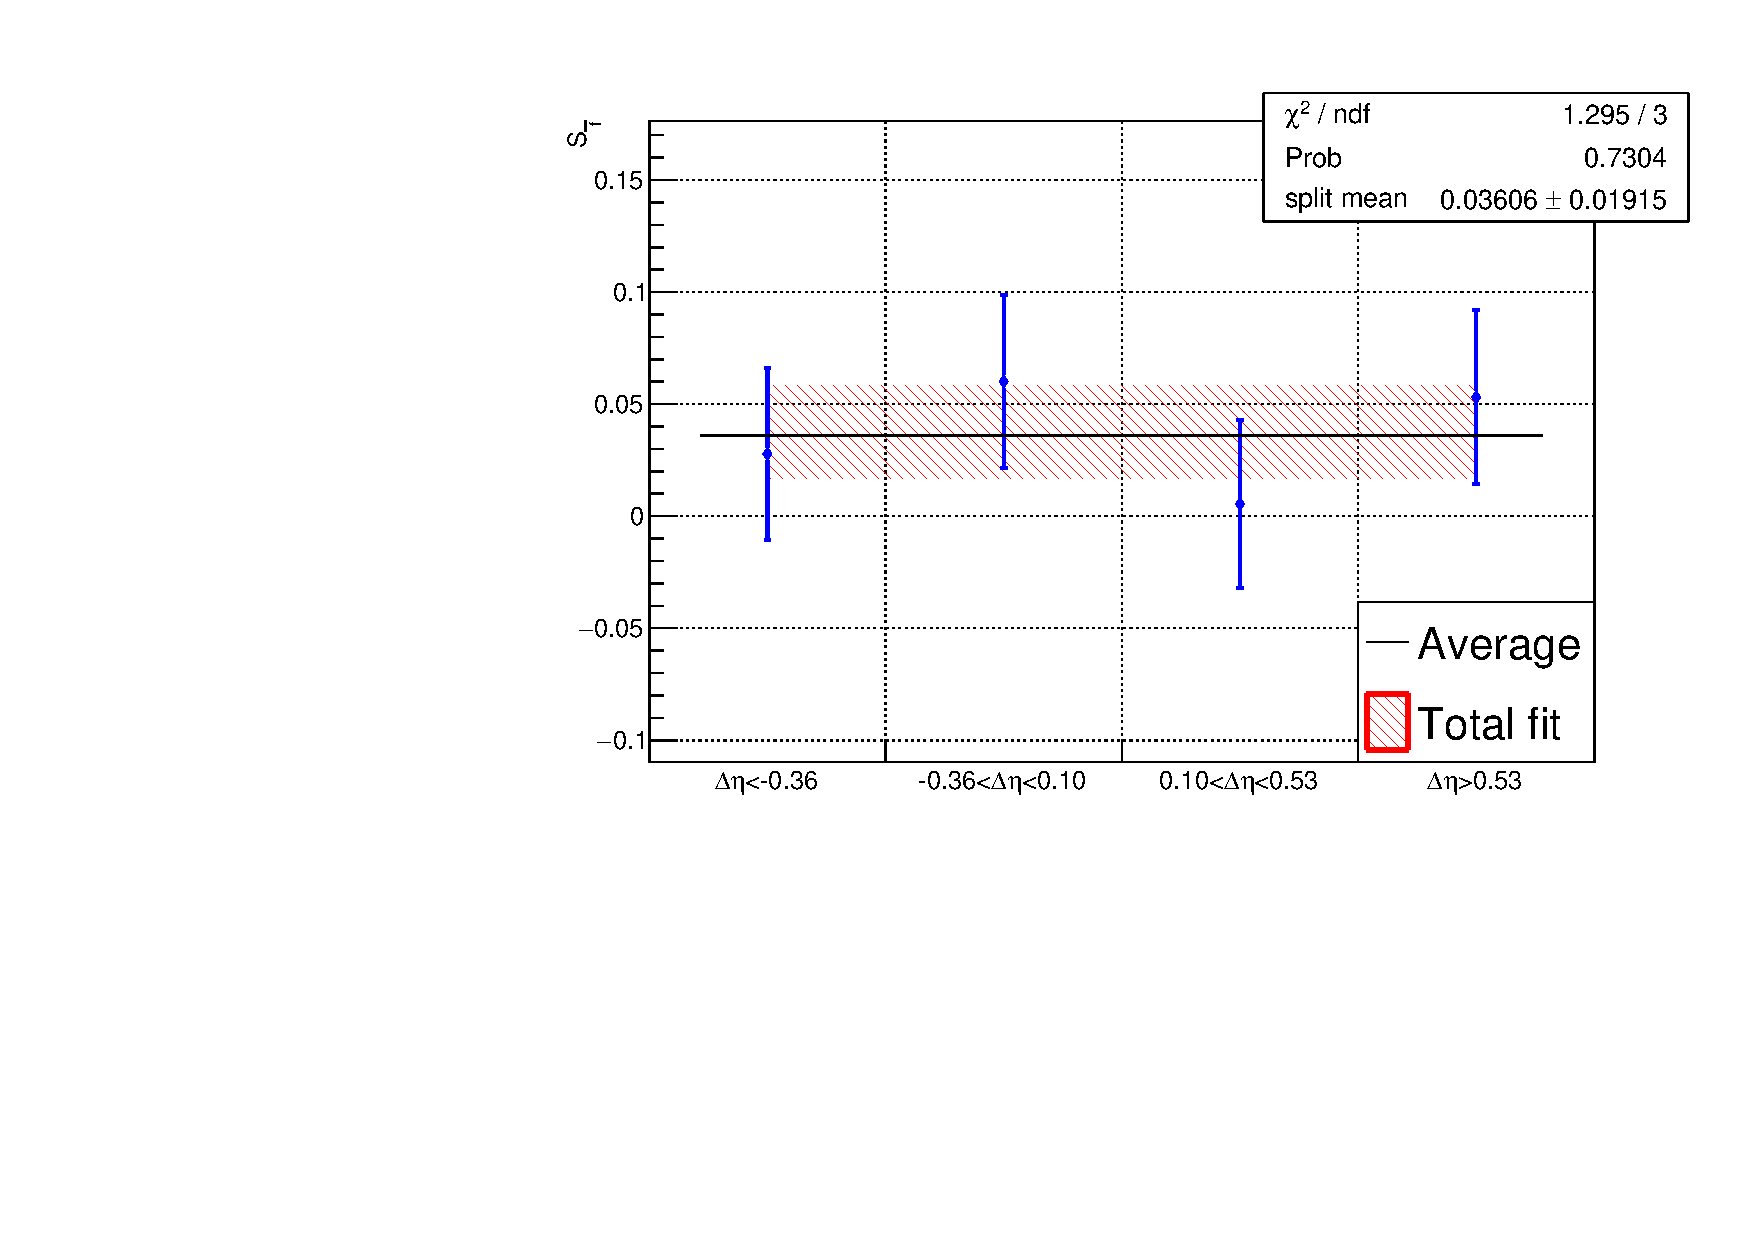
\includegraphics[width=0.45\textwidth]{05DecaytimeFit/figs/splits/Sfbar_splits_DeltaEta.pdf} \\
        \end{center}
        \vspace{-2mm}
        \caption{Fitted values of $S_f$ (left) and $S_{\bar f}$ (right) when the decay time fit is performed
        in bins of (from top to bottom) the transverse momentum of the $\Bz$, number of primary vertices, number of tracks and difference
        in pseudorapidity between the $D$ meson and the bachelor pion. The red hatched band shows the values obtained from the nominal fit of the full sample. The horizontal black line is the result of a $\chi^2$ fit to obtain the weighted average of the results of each subsample.}
        \label{fig:kin_evt_splits}
\end{figure}

Finally, the time fit is repeated separately for TOS candidates on \verb!L0Hadron! and all the other candidates.
The values of $S_{f}$ and $S_{\bar{f}}$ obtained in these subsamples are compared in Fig.~\ref{fig:L0_splits}.
All values are compatible, and no significant dependence of $S_f$ and $S_{\bar f}$ is observed. More details can be found in Appendix~\ref{app:timesplits}.

\begin{figure}[htpb]
        \begin{center}
                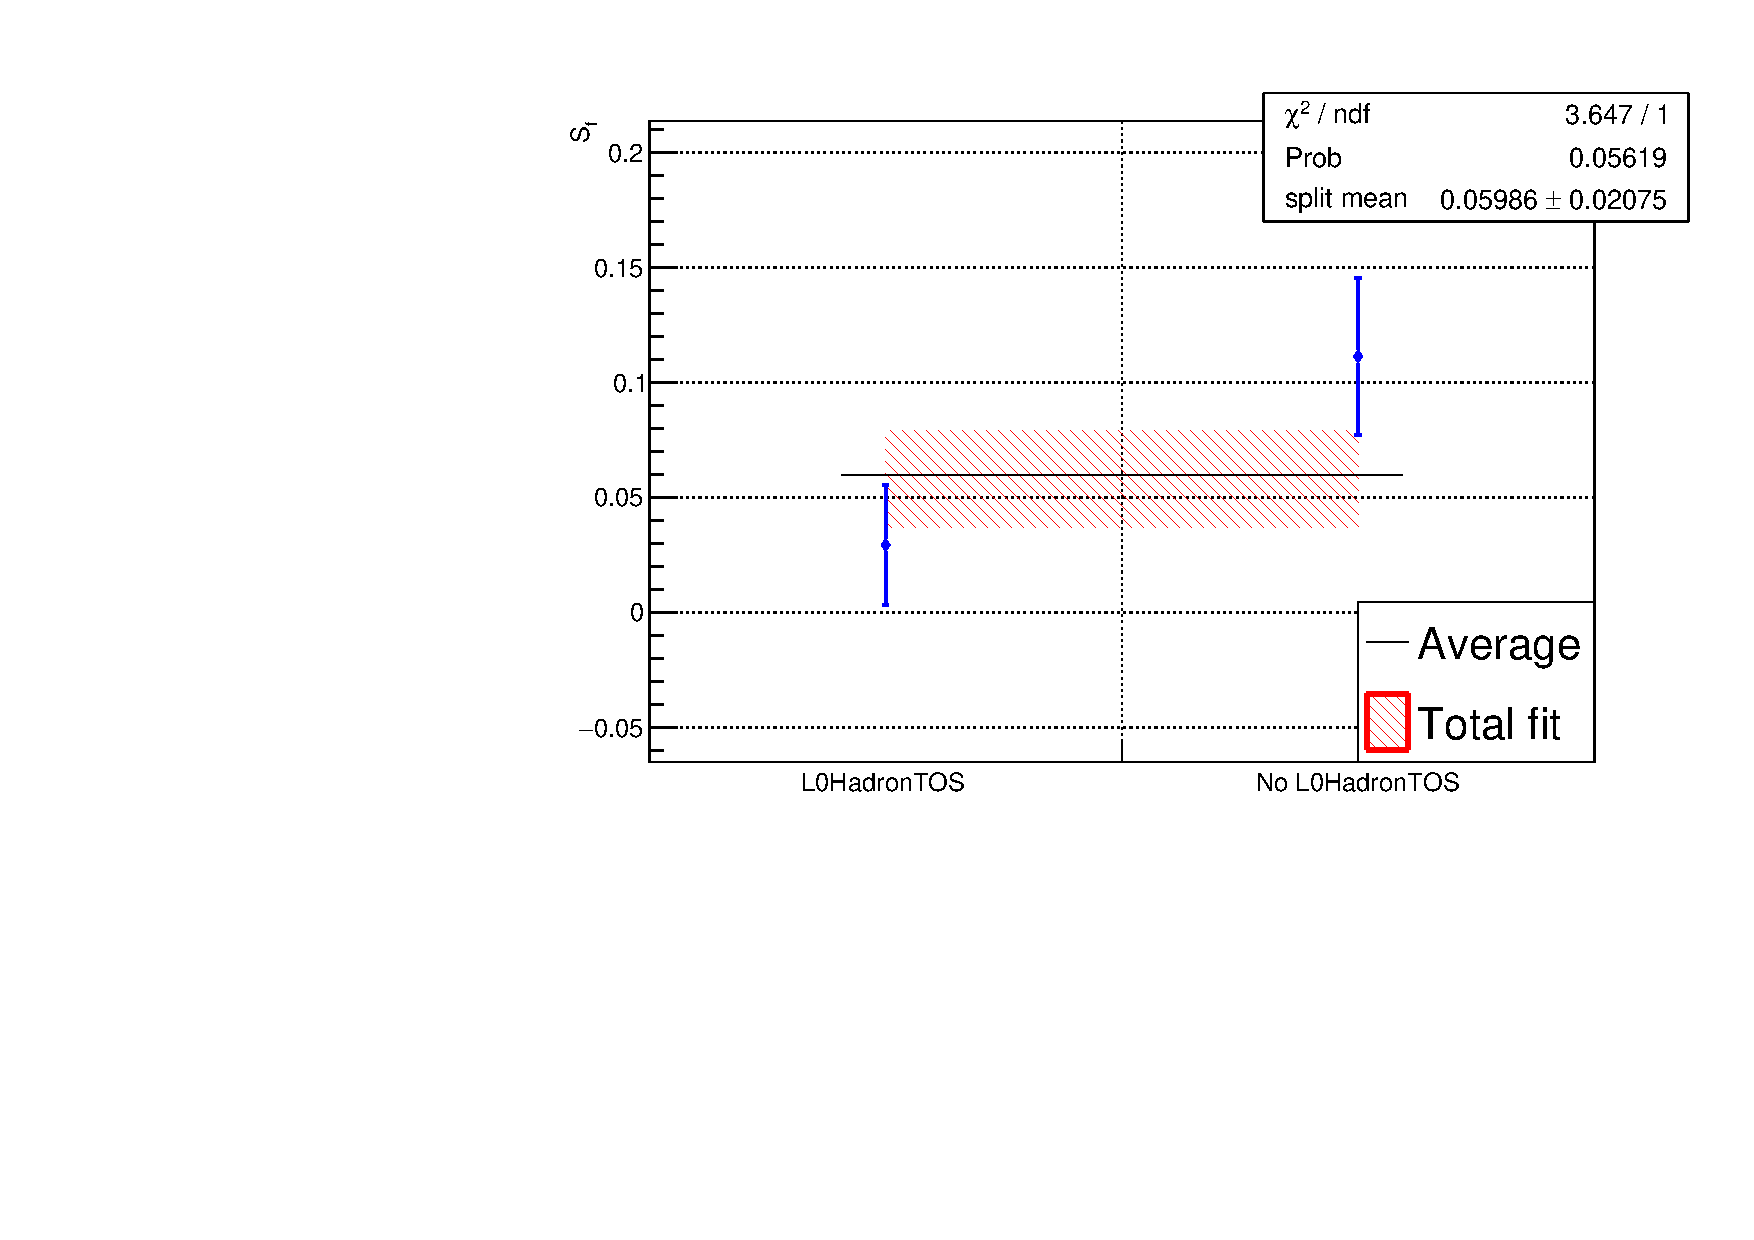
\includegraphics[width=0.49\textwidth]{05DecaytimeFit/figs/splits/Sf_splits_L0HadTos.pdf}
                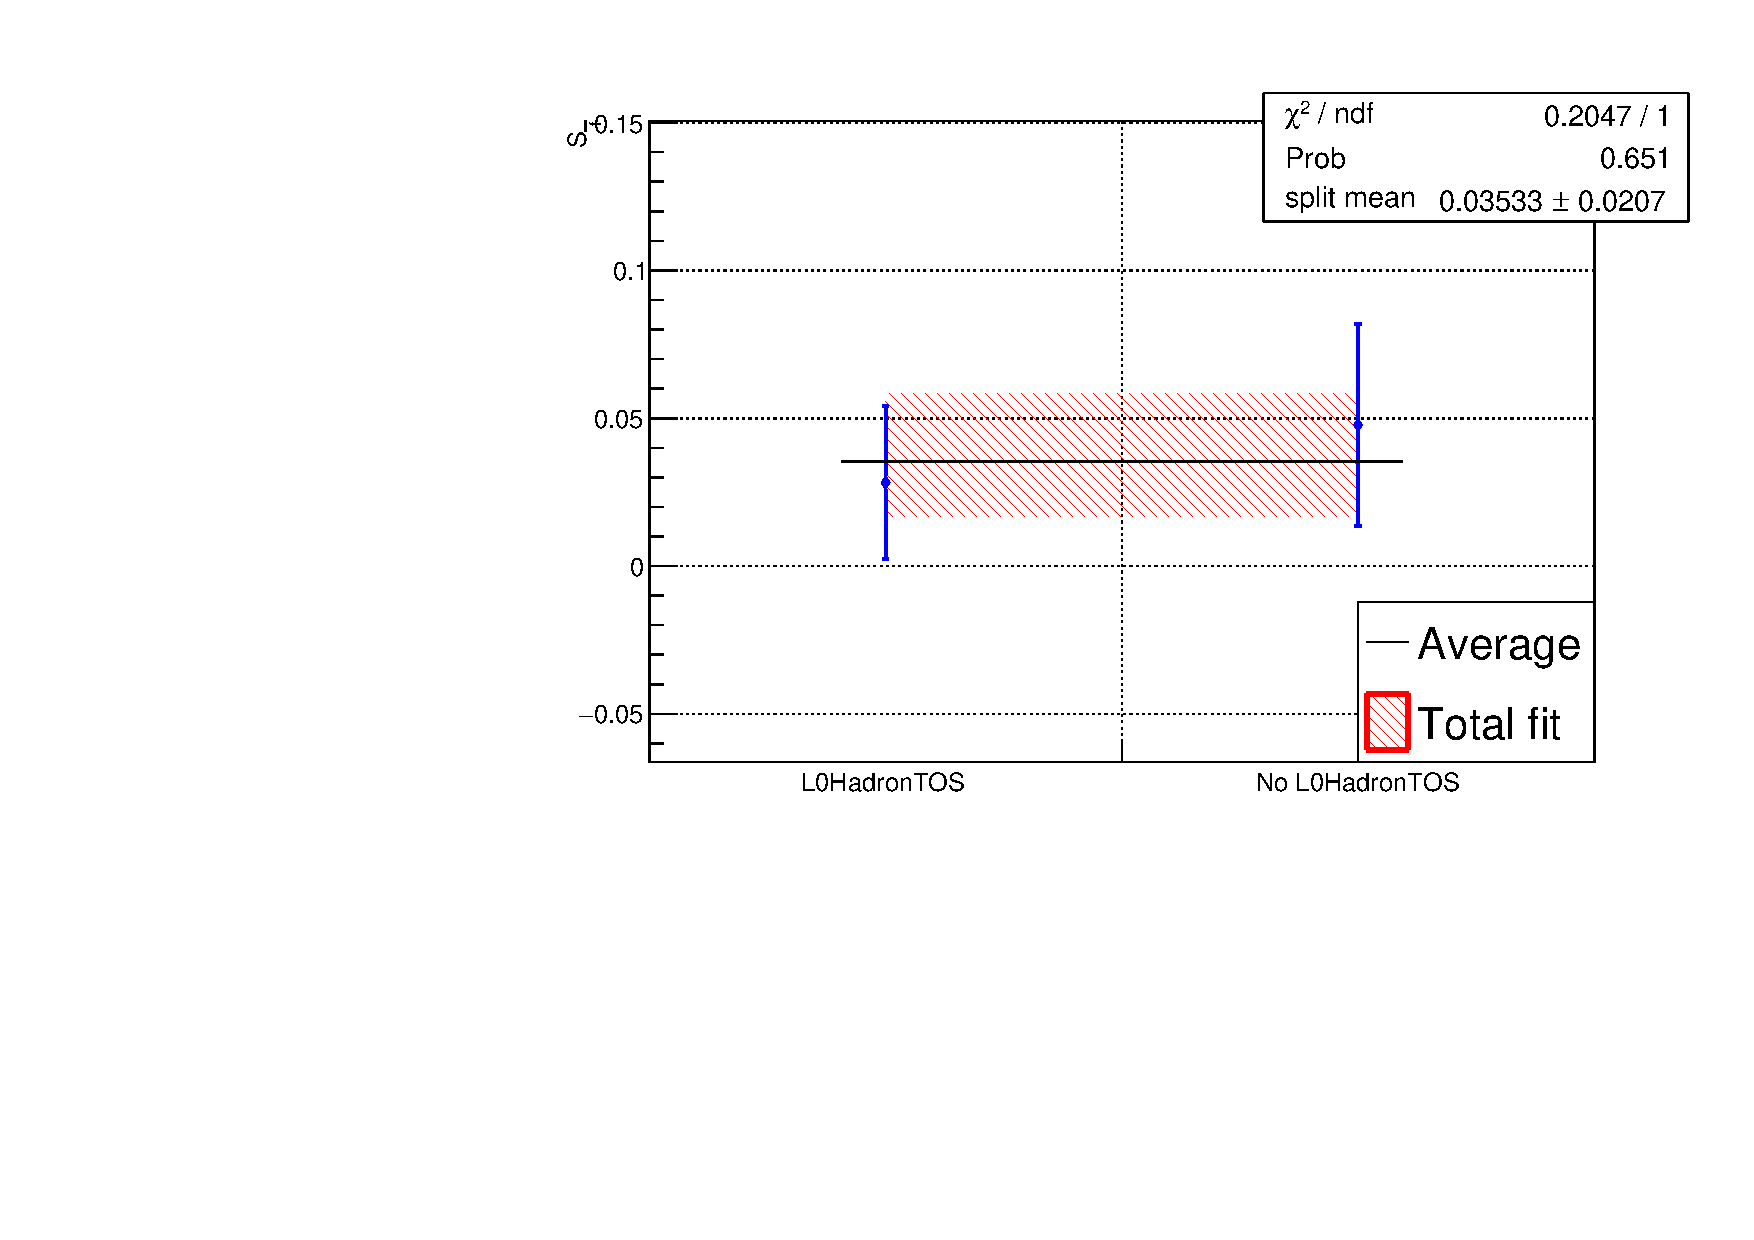
\includegraphics[width=0.49\textwidth]{05DecaytimeFit/figs/splits/Sfbar_splits_L0HadTos.pdf}
        \end{center}
        \vspace{-2mm}
        \caption{Fitted values of $S_f$ (left) and $S_{\bar f}$ (right) when the decay time fit is performed separately for TOS candidates on L0Hadron and all the other candidates.
        The red hatched band shows the values obtained from the nominal fit of the full sample.
        The horizontal black line is the result of a $\chi^2$ fit to obtain the weighted average of the results of each subsample.}
        \label{fig:L0_splits}
\end{figure}

\subsection{Time fits to bootstrapped Monte Carlo samples}
\label{sec:mcbootstrap}
The fit is also validated using Monte Carlo simulation. The $\Bz\to\Dmp\pipm$ simulated sample is \emph{bootstrapped}~\cite{bootstrapping} (\ie,~resampled allowing
repetition of the same candidates) 1000 times. Each bootstrapped sample contains the same signal yield as obtained from
the nominal mass fit (Table~\ref{tab:FitBfloating}), corrected for the \emph{sWeights} dilution factor of
Eq.~\ref{eq:sWeightsDilution} to have the same effective yield as in the data time fit.

Each sample is then fitted using exactly the same strategy as described in Sec.~\ref{sec:datafit}, except
that the central value of the Gaussian constraints on the $\Gamma$ and $\Delta m$ parameters is randomly
drawn from a Gaussian distribution centred on the Monte Carlo generation value given in Appendix~\ref{app:mcgen}
($1/\Gamma=1.519~\rm ps$ and $\Delta m = 0.510~\rm ps^{-1}$) with a standard deviation equal to the 
width of the constraint ($\pm 0.004~\rm ps$ for $1/\Gamma$ and $\pm 0.0023~\rm ps^{-1}$ for $\Delta m$).
This allows
fluctuations of the $\Gamma$ and $\Delta m$ measurements, and avoids underestimation of the fitted uncertainties.

The distributions of the fitted value, uncertainty, pull and residual\footnote{The residual is defined
as fitted value minus generated value, whereas the pull is the residual divided by the fitted uncertainty.} of $S_f$ and
$S_{\bar f}$ are shown in Fig.~\ref{fig:mc_bootstrap_cp}. Other fitted parameters are reported in Appendix~\ref{app:mcbootstrap}. 
Each of these distribution is fitted
with a Gaussian function. The width of the fitted pull distributions are close to unity, meaning that the uncertainty coming from
the likelihood fit is correctly estimated. The mean value of the distribution of the uncertainties of each
parameter is close to the value of the uncertainty found in the fit to data. The on-average better precision found in the fit
to MC is due to the higher tagging performance of the simulation.

The distribution of the residuals of the $S_{f}$ parameter shows a mean of
$0.0071\pm0.0006$, corresponding to one third of the statistical uncertainty of the fit to data;
for $S_{\bar f}$, the mean is $-0.0013\pm0.0006$, which corresponds to about $6\%$ of the statistical uncertainty of the fit to data.

Several configurations are implemented to test the bootstrap study and its results, and to try to address the origin of these
biases. The fits to the bootstrapped samples are repeated in the following different configurations:
\begin{itemize}[noitemsep,topsep=0pt]
\item  using the true flavour of the $\Bz$ candidate instead of the tagging decision and mistag probability: no biases are found
on $S_{f}$ and $S_{\bar f}$;
\item using a \emph{toy} (or \emph{cheated}) tagger, as explained in Appendix~\ref{app:toytagger}: no biases are found on $S_{f}$
and $S_{\bar f}$;
\item using the calibration parameters obtained in the signal MC sample using the true flavour information (see
Sec.~\ref{sec:tagging:OScalib:portability} and Sec.~\ref{sec:tagging:SScalib:portability}): no biases are found on $S_{f}$ and
$S_{\bar f}$;
\item fixing the calibration parameters to the values obtained from the MC samples of the control channels: biases of the order $1\sigma$ on $S_{f}$ and $S_{\bar f}$ are found;
\item applying Gaussian-constraints on the calibration parameters using the values obtained from the MC samples of the control channels: biases
of the order of half the statistical uncertainty of $S_{f}$ and $S_{\bar f}$ are found;
\end{itemize}
This study confirms that the strategy of floating the calibration parameters in the fit is the optimal choice. Other than the
biases related to the flavour-tagging calibrations, the origin of the small bias observed on
the $S_{f}$ parameter in the nominal configuration could not be clarified. To confirm this bias, the study is repeated by fitting additional 1000 bootstrapped
samples using an independent fitter. The mean of the distribution of the residuals in this second study is confirmed to be of the same size,
namely \num{0.0064\pm0.0007} for $S_{f}$ and \num{-0.0024\pm0.0007} for $S_{\bar f}$. Hence, the weighted average of the small residuals
on $S_{f}$ (\num{0.0068\pm0.0005}) and $S_{\bar f}$ (\num{-0.0018\pm0.0005}) of both studies are considered as systematic uncertainties.
As described in Appendix~\ref{app:corrSyst}, the correlation between the systematic uncertainties on $S_{f}$ and $S_{\bar f}$ associated to the fit biases reported here is $0.4$.

\begin{figure}[t]
        \begin{center}
                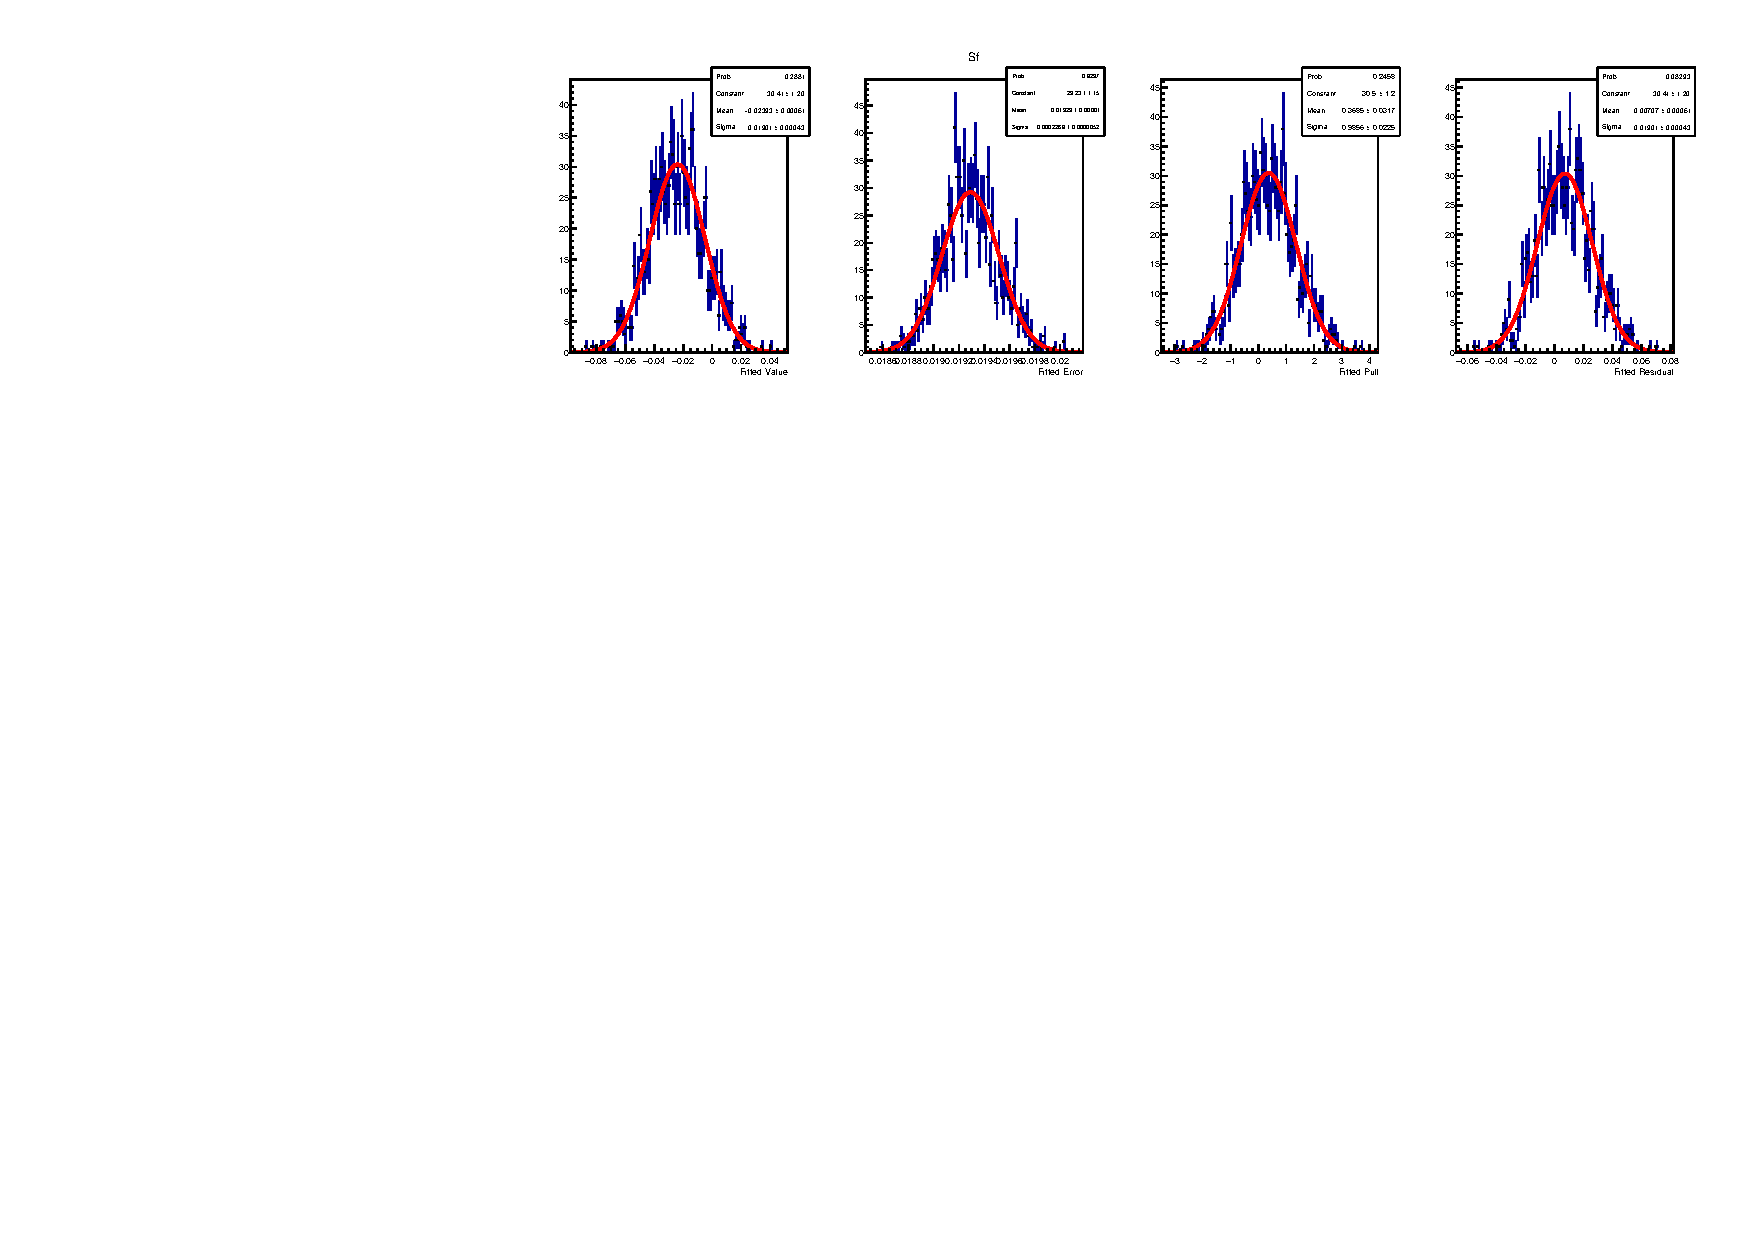
\includegraphics[width=1.0\textwidth]{05DecaytimeFit/figs/MCclosureTest/1DPullPlot_Sf_SSbarAccAsymmFTFloatDMGammaConstrAllSamples.pdf} \\
                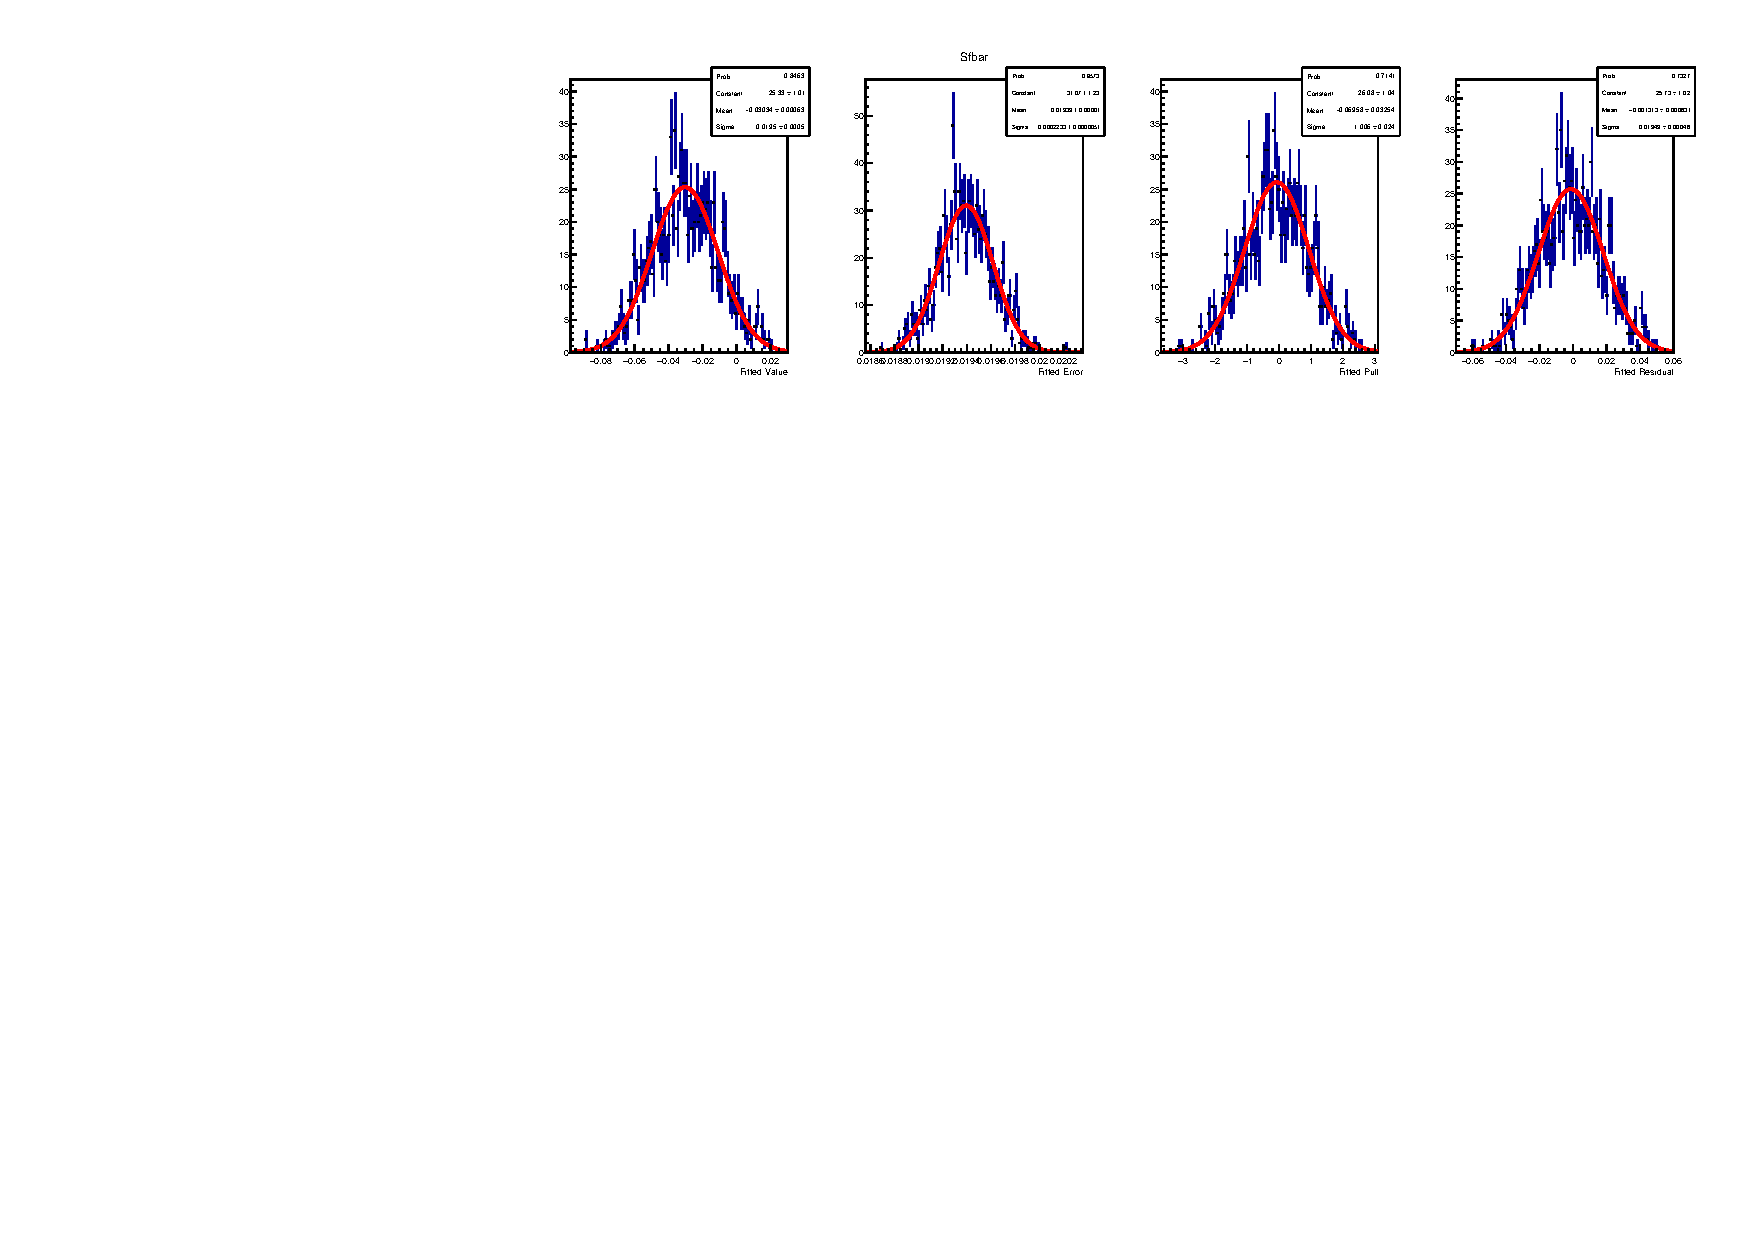
\includegraphics[width=1.0\textwidth]{05DecaytimeFit/figs/MCclosureTest/1DPullPlot_Sfbar_SSbarAccAsymmFTFloatDMGammaConstrAllSamples.pdf}
        \end{center}
        \vspace{-2mm}
        \caption{Distributions of the fitted value, error, pull and residual for $S_f$ (top) and $S_{\bar f}$ (bottom) obtained from
        fits to bootstrapped Monte Carlo samples. Each distribution is fitted with a Gaussian function. Pulls and residuals are computed
        by taking the Monte Carlo generation values as reference (Appendix~\ref{app:mcgen}).}
        \label{fig:mc_bootstrap_cp}
\end{figure}
